\documentclass{article}
\title{Pure Exploration of Combinatorial Bandits}
\author{Shouyuan Chen}
\date{\today}
%%%%%%%%%%%%%%%%%%%%%%%%%%%%%%%%%%%%%%%%%%%%%%%%%%%%%%%%%%%%%

% Change "article" to "report" to get rid of page number on title page
\usepackage{amsmath,amsfonts,amsthm,amssymb}
\usepackage{setspace}
\usepackage{Tabbing}
\usepackage{fancyhdr}
\usepackage{lastpage} 
\usepackage{extramarks}
\usepackage{chngpage}
\usepackage{soul,color}
\usepackage{graphicx,float,wrapfig}
\usepackage{afterpage}
\usepackage{abstract}
\usepackage{hyperref}
\usepackage{natbib}
\usepackage{algpseudocode}
\usepackage{algorithm}
\usepackage{xspace}
\usepackage{subcaption}
\usepackage{theoremref}
% In case you need to adjust margins:
\topmargin=-0.45in
\evensidemargin=0in
\oddsidemargin=0in
\textwidth=6.5in
\textheight=9.0in
\headsep=0.25in

\setlength\parindent{0pt}


% Setup the header and footer
\pagestyle{fancy}
%\lhead{\LatexerName}
%\chead{\LectureClassName: \LectureTitle}
%\rhead{\LectureDate}
%\lfoot{\lastxmark}
%\cfoot{}
\rfoot{Page\ \thepage\ of\ \pageref{LastPage}}
\renewcommand\headrulewidth{0.4pt}
\renewcommand\footrulewidth{0.4pt}

\allowdisplaybreaks

%%%%%%%%%%%%%%%%%%%%%%%%%%%%%%%%%%%%%%%%%%%%%%%%%%%%%%%%%%%%%
% Some tools
\newcommand{\junk}[1]{}

\newtheorem{define}{Definition}
\newtheorem{example}{Example}
\newtheorem{lemma}{Lemma}
\newtheorem{corollary}{Corollary}
\newtheorem{theorem}{Theorem}

\newcommand{\Algorithm}{\texttt{CGapExp}\xspace}
\newcommand{\AlgorithmPAC}{\texttt{CGapExpPAC}\xspace}
\newcommand{\Problem}{\texttt{ExpCMAB}\xspace}
\newcommand{\Rew}{\varphi}
\newcommand{\E}{\mathbb E}

\newcommand{\M}{\mathcal M}
\newcommand{\mmatch}{\mathcal M_{\mathsf{MATCH}}}
\newcommand{\mtop}{\mathcal M_{\mathsf{TOP}m}}
\newcommand{\mbandit}{\mathcal M_{\mathsf{BANDIT}m}}

\newcommand{\diff}{\mathsf{diff}}
\newcommand{\diffvalid}{\prec}
\newcommand{\B}{\mathcal B}
\newcommand{\C}{\mathcal C}
\newcommand{\del}{\backslash}

\newcommand{\RR}{\mathbb R}

%\newcommand{\vec}[1]{\mathbf #1}

\newcommand{\Bopt}{\mathcal B_{\mathsf{opt}}}
\newcommand{\Bmatch}{\mathcal B_{\mathsf{MATCH}}}
\newcommand{\Btop}{\mathcal B_{\mathsf{TOP}m}}
\newcommand{\Bbandit}{\mathcal B_{\mathsf{BANDIT}m}}

\DeclareMathOperator{\rank}{width}
\DeclareMathOperator{\rad}{rad}
\DeclareMathOperator{\decomp}{decomp}
\DeclareMathOperator*{\argmax}{arg\,max}
\DeclareMathOperator*{\argmin}{arg\,min}
\DeclareMathOperator{\Oracle}{Oracle}

\newcommand{\out}{\mathsf{Out}}


\let\Pr\undefined
\DeclareMathOperator{\Pr}{Pr}

\newcommand{\MultiIdent}{\texttt{Multi}\xspace}
\newcommand{\Matroid}{\texttt{Matroid}\xspace}
\newcommand{\Match}{\texttt{Match}\xspace}
\newcommand{\Path}{\texttt{Path}\xspace}

\newcommand{\inn}[1]{\left\langle #1 \right\rangle}
\newcommand{\nor}[1]{\left\|#1\right\|}
\renewcommand{\vec}[1]{\boldsymbol{#1}}

\renewcommand{\odot}{\circ}

%%%%%%%%%%%%%%%%%%%%%%%%%%%%%%%%%%%%%%%%%%%%%%%%%%%%%%%%%%%%%

\begin{document}
\begin{spacing}{1.1}
\newpage

\maketitle


\section{Introduction}

\subsection{Related Work}

\textbf{Notations.} 

\section{Pure Exploration of Combinatorial Bandits}


%Let $\vec u \in \RR^{n}$ be a vector. 
% and $M\subseteq [n]$ be a set. 

\textbf{\Problem: problem formulation.}
Suppose that there are $n$ arms and the arms are numbered $1,2,\ldots,n$.
Each arm $e\in[n]$ is associated with a reward distribution $\Rew_e$ and define $w(e)=\E_{X\sim \Rew_e}[X]$ be the expected reward. 
Let $\vec w = \big(w(1),\ldots, w(n)\big)^T$ denote the vector of expected rewards.

Let $\M\subseteq 2^{[n]}$ be the family of all feasible solutions to a combinatorial problem.
%Let $M_* = \argmax_{M\in \M} w(M)$ denote the optimal set of arms which max
A learner wants to find the optimal solution of $\M$ which maximizes the expected reward $M_*=\argmax_{M\in \M} w(M)$ by playing the following game.
%The learning problem of pure exploration combinatorial bandit can be formalized as a game between a learner and a stochastic environment, where the learner's goal is to find the optimal solution to the combinatorial problem which maximizes the sum of expected reward $M_* = \argmax_{M\in \M} w(M)$.
At the beginning of the game, the reward distributions $\{\Rew_e\}_{e\in[n]}$ are unknown to the learner.
Then, the game is played for multiple rounds;
on each round $t$, the learner pulls an arm $p_t\in [n]$ and observes a reward sampled from the associated reward distribution $\Rew_{p_t}$.
The game continues until certain stopping condition is satisfied.
%which will be specified later.
After the game finishes, the learner need to output a solution $\out \in \M$.
%For the sake of simplicity, we shall assume that the optimal set $M_*$ is unique throughout the paper.

%Let $n$ denote the number of arms and suppose that the arms are numbered $1,2,\ldots,n$.

%We assume that all reward distributions are $R$-sub-Gaussian [].
%Notice that all distributions that are supported on $[0,R]$ are $R$-sub-Gaussian distributions [] and therefore our model subsumes the cases of bounded rewards.
%Let $w(e)=\E_{X\sim \Rew_e}[X]$ denote the expected reward of arm $e$ and let $\vec w = \big(w(1),\ldots,w(n)\big)^T$ denote the vector of expected rewards.
%In addition, for any set of arms $M\subseteq [n]$, we define $w(M) = \sum_{e\in M} w(e)$ as the sum of expected rewards of arms that belong to $M$.

%Notice that, if $\epsilon = 0$, then the learner is required to identify the optimal set, i.e. $\out = M_*$.



%\textbf{Fixed confidence and fixed budget.} 
We consider two different stopping conditions of the game, which are known as \emph{fixed confidence} setting and \emph{fixed budget} setting.
In the fixed confidence setting, the learner can stop the game at any point and her goal is to achieve a fixed confidence about the optimality of the returned set while uses a small number of pulls.
Specifically, given a confidence parameter $\delta$, the learner need to guarantee that $\Pr[\out = M_*] \ge 1-\delta$.
The performance is evaluated by the number of pulls used by the learner.
%Notice that the learner can stop the game at any point in this setting.
In the fixed budget setting, the game stops after a fixed number rounds.
The learner tries to minimize the probability of error $\Pr[\out \not= M_*]$ within these rounds.
In this case, the learner's performance is measured by the probability of error.


\textbf{Examples of combinatorial problems.} 
The formulation of the \Problem problem covers many online learning tasks.
We consider the following problems as examples.
\begin{itemize}
\item \MultiIdent.
\item \Matroid.
\item \Match.
\item \Path.
\end{itemize}

We assume that all reward distributions have $R$-sub-Gaussian tails. 
Formally, for each $e\in [n]$, let $X_e$ be an independent sample of $\Rew_e$. 
Then, for all $t\in \RR$, we have $\exp\big(t (X_e-w(e) \big) \le \exp(R^2t^2/2)$.
It is well known that all distributions that are supported on $[0,R]$ satisfy by this assumption [].
Finally, for the sake of simplicity, we will assume that the optimal solution $M_*$ is unique.

%\textbf{Useful notations.}
%For any vector $\vec v\in \RR^n$ and any set $M \subseteq [n]$, we define $v(M) = \sum_{e\in M} v(e)$.


\section{Algorithm and Main Result}
%Our main contribution is an algorithm for solving the \Problem problem.
%Our algorithm 

%In this section, we describe our algorithm for pure exploration combinatorial bandit problem.
%Then, we analyze the sample complexity and the probability of error of our algorithm.

In this section, we present \Algorithm, a learning algorithm for the \Problem problem in the fixed confidence setting, and analyze its sample complexity. 
%Then, we analyze the sample complexity of \Algorithm algorithm.
The \Algorithm algorithm can be extended to the fixed budget and PAC learning settings. 
We will discuss these extensions in Section~\ref{section:extensions}.

%Many common combinatorial problems admit computationally efficient oracles.

\textbf{Oracle.}
We allow the \Algorithm algorithm to access a \emph{maximization oracle}. 
A maximization oracle takes a weight vector $\vec v \in \RR^{n}$ as input and computes an optimal solution with respect to the weight vector $\vec v$.
Formally, we call a function $\text{Oracle:}~\RR^{n} \rightarrow \M$ a maximization oracle if $\Oracle(\vec v) \in \argmax_{M\in \M} v(M)$ for all $\vec v\in \RR^{n}$.
It is clear that a very broad class of combinatorial problems admit such maximization oracles.
Besides the access to the oracle, \Algorithm does not need \emph{any} additional knowledge of the combinatorial problem $\M$.

%For most non-trivial combinatorial problems, the size of the collection of feasible sets $\M$ is exponential in $n$.
%Hence, the definition of $\M$ 
%Therefore, the learning algorithm needs a succinct representation of $\M$.
%In particular, we allow the learning algorithm to use a \emph{maximization oracle} which can find the optimal set $M\in \M$ when the expected reward of each arm is known.
%Specifically, we assume that there exists an oracle which takes a vector $\vec v = \big(v(1),\ldots,v(n)\big)^T$ as input and returns a set $\Oracle(\vec v) = \argmax_{M\in \M} v(M)$.


\textbf{Algorithm.} 
%
%Our algorithm works for both fixed confidence and fixed budget settings.
%In either settings, the behaviors of our algorithm only differ in the construction of confidence radius and the stopping condition.
%In the following, we describe the procedure of our algorithm.
The \Algorithm algorithm maintains empirical mean $\bar w_t(e)$ and confidence radius $\rad_t(e)$ for each arm $e\in[n]$ and each round $t$.
The construction of confidence radius ensures that $|w(e)-\bar w_t(e)| \le \rad_t(e)$ holds with high probability for each arm $e \in [n]$ and each round $t>0$.
\Algorithm begins with an initialization phase in which each arm is pulled once.
Then, at round $t \ge n$, \Algorithm uses the following procedure to find an arm to pull. 
First, \Algorithm calls the oracle which computes the solution $M_t=\Oracle(\vec {\bar w}_t)$. 
The solution $M_t$ is the ``best'' solution with respect to the empirical means $\vec {\bar w}_t$.
% which maximizes empirical means $\bar w_t$ up to  $t$.
Then, \Algorithm explores possible refinements of $M_t$. 
In particular, \Algorithm uses the confidence radius to compute an adjusted expectation vector $\vec {\tilde w}_t$ in the following way: for each arm $e \in M_t$, $\tilde w_t(e)$ equals to the lower confidence bound $\tilde w_t(e) = \bar w_t(e)-\rad_t(e)$; and for each arm $e\not\in M_t$, $\tilde w_t(e)$ equals to the upper confidence bound $\tilde w_t(e)=\bar w_t(e)+\rad_t(e)$.
Intuitively, the adjusted expectation vector $\vec {\tilde w}_t$ penalizes arms belonging to the current solution $M_t$ and encourages exploring arms out of $M_t$.
\Algorithm then calls the oracle using the adjusted expectation vector $\vec {\tilde w}_t$ as input to compute a refined solution $\tilde M_t = \Oracle(\vec {\tilde w}_t)$.
If $\tilde w_t(\tilde M_t) = \tilde w_t(M_t)$ then \Algorithm stops and returns $\out=M_t$.
Otherwise, \Algorithm pulls the arm belonging to the symmetric difference $(\tilde M_t \del M_t) \cup (M_t \del \tilde M_t)$ between $M_t$ and $\tilde M_t$ with the largest confidence radius in the end of round $t$.
The pseudo-code of \Algorithm is shown in Algorithm~\ref{algo:pac}. 


\begin{algorithm}[htbp]
\begin{algorithmic}[1]
\Require Confidence parameter: $\delta \in (0,1)$; Maximization oracle: $\Oracle(\cdot): \RR^n \rightarrow \M$.
\Statex \textbf{Initialize:} Play each arm $e \in [n]$ once. Initialize empirical means $\vec {\bar w}_n$ and set $T_{n}(e) \gets 1$ for all $e$.
\For{$t=n,n+1,\ldots$}
	\State $M_t \gets \Oracle(\vec {\bar w}_t)$
	\For{$e\in [n]$}
		\If {$e\in M_t$}
			\State $\tilde w_t(e) \gets \bar w_t(e)-\rad_t(e)$
		\Else
			\State $\tilde w_t(e) \gets \bar w_t(e)+\rad_t(e)$
		\EndIf
	\EndFor
	\State $\tilde M_t \gets \Oracle(\vec{\tilde w}_t)$
	\If{$\tilde w_t(\tilde M_t) = \tilde w_t(M_t)$}
		\State $\out \gets M_t$
		\State \textbf{return} $\out$
	\EndIf
	\State $p_t \gets \argmax_{e\in (\tilde M_t \del M_t) \cup (M_t \del \tilde M_t)} \rad_t(e)$\label{algo:step:D}
	\State Pull arm $p_t$ and observe the reward
	\State Update empirical means $\vec {\bar w}_{t+1}$ using the observed reward
	\State Update number of pulls: $T_{t+1}(p_t)\gets T_{t}(p_t)+1$ and $T_{t+1}(e) \gets T_{t}(e)$ for all $e\not=p_t$
	\EndFor
\end{algorithmic}
\caption{\Algorithm: Combinatorial Gap Exploration}
\label{algo:pac}
\end{algorithm}


\subsection{Analysis}
%In this part, we analyze the performance of Algorithm~\ref{algo:pac} for both fixed confidence and fixed budget settings. 


\textbf{Gap.} We begin with defining a natural complexity measure of the \Problem problem. 
For each arm $e \in [n]$, we define gap $\Delta_e$ as
\begin{equation}
\label{eq:define-delta}
\Delta_e = \begin{cases}
			   w(M_*)-\max_{M\in \M: e\in M} w(M) & \text{if } e\not \in M_*, \\
			   w(M_*)-\max_{M\in \M: e\not \in M} w(M) & \text{if } e\in M_*,
			\end{cases}
\end{equation}
where we use the convention that the maximum value of an empty set is $-\infty$.
We also define $\mathbf H$ as the sum of inverse squared gaps 
$$
\mathbf H =\sum_{e\in [n]} \Delta_e^{-2}.
$$

From Eq.~\eqref{eq:define-delta}, we see that, for each arm $e\not\in M_*$, $\Delta_e$ represents the gap between the optimal set $M_*$ and the best set that includes arm $e$; and, for each arm $e\in M_*$, $\Delta_e$ is the sub-optimality of the best set that does not include arm $e$.
%We notice that, for many combinatorial problems, the definition Eq.~\eqref{eq:define-delta} naturally reflects the hardness of an arm.
%().
%Figure X illustrates these interpretations.
We notice that this definition resembles the definition of gaps for \MultiIdent proposed by ().



\textbf{Exchange class.} 
The analysis of our algorithm depends on certain exchange properties of combinatorial structures.
To capture these properties, we introduce notions of \emph{exchange set} and \emph{exchange class} as tools for our analysis.
We present their definitions in the following.

%An exchange set is defined as a pair of disjoint sets.

We begin with the definition of exchange set. 
We define an exchange set $b$ as an ordered pair of disjoint sets $b=(b_+,b_-)$.
Then, we define operator $\oplus$ such that, for any set $M$ and any exchange set $b=(b_+,b_-)$, we have $M\oplus b \triangleq M\del b_- \cup b_+$.
Similarly, we also define operator $\ominus$ such that $M\ominus b \triangleq M\del b_+\cup b_-$.

We call a family of exchange sets $\B$ an \emph{exchange class for $\M$} if $\B$ satisfies the following property.
Let $M$ and $M'$ be two  elements of $\M$.
Then, for any $e \in (M\del M')$, there exists an exchange set $(b_+,b_-)\in \B$ which satisfies $e\in b_-$, $b_+ \subseteq M'\del M$, $b_- \subseteq M \del M'$, $(M\oplus b) \in \M$ and $(M'\ominus b) \in \M$.
Finally, we define the \emph{width} of exchange class $\B$ as follows
\begin{equation}
\label{eq:width}
\rank(\B) = \max_{(b_+,b_-) \in \B} |b_+|+|b_-|.
\end{equation}

%An exchange class can be seen as a set operations that transform one feasible set to another.

Intuitively, for any feasible sets $M$ and $M'$, there exists an exchange set $(b_+,b_-)\in \B$ belonging to the exchange clas $\B$ which can be seen as an ``operation'' that transforms $M$ one step towards $M'$: this operation generates a new feasible set $M\oplus b$ by removing elements (including $e$) from $M$ and adding elements which belongs to $M'$.
%Therefore, for any two elements $M,M'$ of $\M$, one can sequentially apply a finite number of these operations of $\B$ to transform $M$ to $M'$.it
One can chain these operations together such that, for any $M\not= M'$, there exists a sequence of exchange sets $b_1,\ldots, b_k$ of $\B$ such that $M'=M\oplus b_1 \oplus \ldots \oplus b_k$.

We notice that an exchange class for $\M$ can be ``redundant'' by our definition, i.e. it may contains some unnecessary exchange set $b$, such that $M\oplus b \not\in \M$ for any $M \in \M$.
These redundant exchange sets do not affect our analysis.
But allowing them would simplify the construction and description of exchange classes for certain combinatorial problems.
%On the other hand, this also means that, for a fixed combinatorial problem, there exist many exchange classes.
%In particular, we are interested with the exchange classes with small widths.

\junk{
Next, we investigate the exchange classes for our running examples.
For \MultiIdent problem, we can construct the exchange class as $\B_{1}=\{(\{i\},\{j\})\;|\;\forall i\in [n], j\in [n]\}$.
It is easy to verify $\B_{1}$ is an exchange class for $\M_{\MultiIdent}$: one can transform a set of $k$ elements to another by adding and removing an element for each time.
In fact, a standard result from matroid theory, called basis exchange property (see Lemma~\ref{lemma:basis-exchange-matroid} in the appendix), shows that $\B_1$ is also an exchange class for the more general \Matroid problem.
%From Lemma~\ref{lemma:basis-exchange-matroid}, we see that $\B_1$ is an exchange class for $\M_{\Matroid}$.
Next, for \Match problem, an exchange class contains all cycles of the graph $G$.
Given two matchings $M,M'$, the union $M\cup M'$ is a union of disjoint cycles [].
These cycles are known to be augmenting cycles in combinatorial optimization literature [].
Figure~Y illustrates these exchanges classes.
}

Next, we construct the exchange classes for our running examples. 
Our constructions are summarized in Lemma~\ref{lemma:example-exchange-class}.
\begin{lemma}
There exist exchange classes $\B_{\MultiIdent}$, $\B_{\Matroid}$, $\B_{\Match}$ and $\B_{\Path}$ for $\M_{\MultiIdent}$, $\M_{\Matroid}$, $\M_{\Match}$ and $\M_{\Path}$, respectively. 
These exchange classes can be constructed as follows
\begin{enumerate}
	\item $\B_{\MultiIdent}=\big\{(\{i\},\{j\})\;|\;\forall i\in [n], j\in [n]\big\}$.
	\item $\B_{\Matroid}=\big\{(\{i\},\{j\})\;|\;\forall i\in [n], j\in [n]\big\}$.
	\item $\B_{\Match}=\big\{(C_+,C_-)\;|\; C_+\cup C_- \text{ is a cycle of }G\big\}$.
	\item $\B_{\Path}=\big\{ (P_1, P_2) \;|\;P_1,P_2\text{ are two disjoint paths of }G\text{ with same endpoints}\big\}$.
\end{enumerate}
In addition, we have $\rank(\B_{\MultiIdent})=2$, $\rank(\B_{\Matroid})=2$, $\rank(\B_{\Match})=|V|$ and $\rank(\B_{\Path})=|V|$.
\label{lemma:example-exchange-class}
\end{lemma}
The  construction for \MultiIdent problem is straightforward.
For \Matroid problem, we leverage the basis exchange property of matroids (see Lemma~\ref{lemma:basis-exchange-matroid} in the appendix).
And for \Match and \Path problems, we appeal to  graph-theoretical properties of matchings and paths.
We illustrate elements of these  exchanges classes in \autoref{fig:exchange}.
A detailed proof of Lemma~\ref{lemma:example-exchange-class} is deferred to the supplementary material.

\begin{figure}
\centering
\begin{subfigure}[c]{0.22\textwidth}
	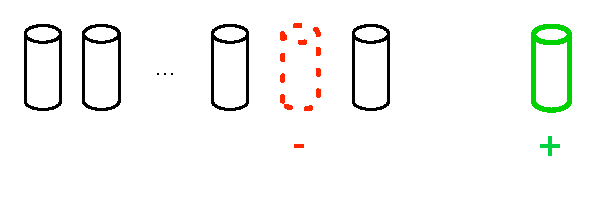
\includegraphics[width=\textwidth]{fig/exchange-multi}
	\caption{An element of $\B_{\MultiIdent}$.}
\end{subfigure}
~
\begin{subfigure}[c]{0.25\textwidth}
	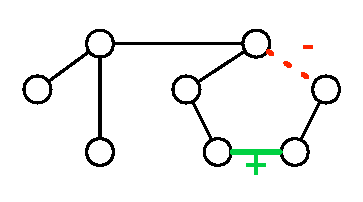
\includegraphics[width=\textwidth]{fig/exchange-matroid}
	\caption{An element of $\B_{\Matroid}$}
	\label{fig:exchange:matroid}
\end{subfigure}
~
\begin{subfigure}[c]{0.22\textwidth}
	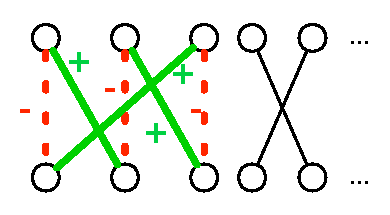
\includegraphics[width=\textwidth]{fig/exchange-match}
	\caption{An element of $\B_{\Match}$.}
\end{subfigure}
~
\begin{subfigure}[c]{0.22\textwidth}
	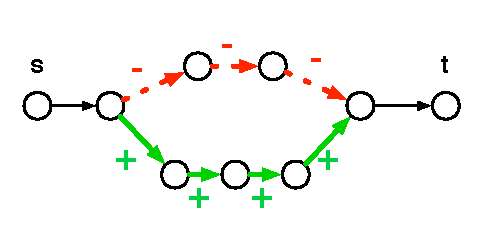
\includegraphics[width=\textwidth]{fig/exchange-path}
	\caption{An element of $\B_{\Path}$.}
\end{subfigure}
\caption{
Examples of exchange sets belonging to the exchange classes $\B_{\MultiIdent}$, $\B_{\Matroid}$, $\B_{\Match}$ and $\B_{\Path}$:
green-solid elements constitute the set $b_+$, red-dotted elements constitute the set $b_-$ and the example exchange set is $b=(b_+,b_-)$. 
(In \autoref{fig:exchange:matroid}, we consider spanning tree as a specific instance for the \Matroid problem.)
}
\label{fig:exchange}
\end{figure}

\textbf{Main result.} 
Our main result is a problem-dependent sample complexity bound of the \Algorithm algorithm.
In particular, we show that \Algorithm returns the optimal set with high probability and uses at most $\tilde O\big(\rank(\B)^2 \mathbf H\big)$ samples.
\begin{theorem}
Given any $\delta \in (0,1)$, any combinatorial problem $\M \subseteq 2^{[n]}$ and any vector $\vec w \in \RR^{n}$.
Assume that the reward distribution $\Rew_e$ for each arm $e\in [n]$ is  $R$-sub-Gaussian with mean $w(e)$.
Let $\B$ be an exchange class for $\M$ and let $\{\Delta_e\}_{e\in [n]}$ be the gaps defined in Eq.~\eqref{eq:define-delta}.

Set $\rad_t(e) = R\sqrt{\frac{2\log\left(\frac{4n t^2}\delta\right)}{T_e(t)}}$ for all $t > 0$ and $e\in[n]$.
Then, with probability at least $1-\delta$, the \Algorithm algorithm (Algorithm~\ref{algo:pac}) returns the optimal set $\out=M_*$ and
\begin{equation}
\label{eq:sample-complexity}
T \le O\left(R^2\rank(\B)^2\mathbf H\log\left(R^2\rank(\B)^2\mathbf H \cdot n/\delta\right)\right),
\end{equation}
where $T$ denotes the number of samples used by Algorithm~\ref{algo:pac}.
\label{theorem:main}
\end{theorem}

\textbf{Remarks.}
%Theorem~\ref{theorem:main} upper bounds the sample complexity of \Algorithm for an arbitrary combinatorial problem $\M$.
%We see that the sample complexity Eq.~\eqref{eq:sample-complexity} depends on $\rank(\B)$ and $\B$ is an arbitrary exchange class for $\M$.
%Therefore, the sample complexity Eq.~\eqref{eq:sample-complexity} is minimizes $\B$ 
%Notice that $\B$ does not 
%Theorem~\ref{theorem:main} is a general result which provides a sample complexity for any combinatorial problem $\M$.
For the \MultiIdent problem, we see that Lemma~\ref{lemma:example-exchange-class} indicates that $\B_{\MultiIdent}$ is an exchange class for $\M_{\MultiIdent}$ and $\rank(\B_{\MultiIdent})=O(1)$.
Therefore, the sample complexity bound of \Algorithm for the \MultiIdent problem is $O\big(\mathbf H \log(n\mathbf H/\delta)\big)$.
This matches the previous known problem-dependent bounds for the \MultiIdent problem due to XXX [] within logarithmic factors.
%And Theorem~\ref{algo:pac} establishes the first sample complexity bound for the pure exploration of other combinatorial bandits.
For the \Matroid problem, we know that $\B_{\Matroid}=O(1)$ and hence the sample complexity is also $O\big(\mathbf H \log(n\mathbf H/\delta)\big)$.
Finally, for \Match and \Path problem, we see that the sample complexity is bounded by $\tilde O(|V|^2 \mathbf H)$.



%Many combinatorial problem $\M$ is associated with an exchange class with small width.


%From the definition, it is easy to see that if $\B$ is an exchange class, then, for any $M\not= M'$, there exists a sequence of exchange sets $b_1,\ldots, b_k$ belonging to $\B$ such that $M'=M\oplus b_1 \ldots \oplus b_k$.
%Hence, intuitively, an exchange class for $\M$ characterizes the ``operations'' of transforming an element $M\in \M$ to another element $M'\in \M$.



\section{Lower Bounds}

In this section, we prove a problem-dependent lower bound on the sample complexity of the \Problem problem. 
To state our results, we first define the notion of \emph{$\delta$-correct algorithm} as follows.
For any $\delta \in (0,1)$, we call an algorithm $\mathbb A$ a $\delta$-correct algorithm if, for any expected reward $\vec w \in \RR^{n}$, the probability of error of $\mathbb A$ is at most $\delta$, i.e. $\Pr[M_*\not =\out] \le \delta$, where $\out$ is the output of algorithm $\mathbb A$.

We show that, for any combinatorial problem $\M$ and any expected rewards $\vec w$, any $\delta$-correct algorithm $\mathbb A$ must use at least $\Omega\big(\mathbf H \log(1/\delta) \big)$ samples in expectation.
\begin{theorem}
Fix any $\M\subseteq 2^{[n]}$ and any vector $\vec w \in \RR^n$.
Suppose that, for each arm $e\in [n]$, the reward distribution $\Rew_e$ is given by $\Rew_e=\mathcal N(w(e),1)$, where $\mathcal N(\mu, \sigma^2)$ denotes a Gaussian distribution with mean $\mu$ and variance $\sigma^2$. 
Then, for any $\delta \in (0,e^{-16}/4)$ and any $\delta$-correct algorithm $\mathbb A$, we have
\begin{equation}
\label{eq:lower-bound}
\E[T] \ge \frac{1}{16} \mathbf H \log\left(\frac{1}{4\delta}\right),
\end{equation}
where 
$T$ denote the number of total samples used by algorithm $\mathbb A$ and
$\Delta_e$ is defined in Eq.~\eqref{eq:define-delta}.
\label{theorem:lower-bound}
\end{theorem}

%Now we compare the sample complexity Eq.~\eqref{eq:sample-complexity} of \Algorithm to the lower bound provided in Theorem~\ref{theorem:lower-bound} on our running examples \MultiIdent, \Matroid, \Match and \Path.
%For clarity, we consider the case that $\epsilon=0$ which corresponds to the learning problem of finding the optimal set.
%We see that \Algorithm algorithm uses at most $\tilde O(\rank(\B)^2 \mathbf H)$ samples.
%Recall that, for \MultiIdent and \Matroid, Lemma~\ref{lemma:example-exchange-class} shows that $\rank(\B)=2$.
Recall that, for the \MultiIdent problem and the \Matroid problem, the sample complexity of \Algorithm is $O(\mathbf H\log(n\mathbf H/\delta))$.
Hence, for these two problems, the \Algorithm algorithm achieves the optimal sample complexity within logarithmic factors.
In addition, our result confirms the conjecture of XXX [] that the lower bound of sample complexity of \MultiIdent problem is $\Omega\big(\mathbf H\log(1/\delta)\big)$.

%On the other hand, for $\Match(V,E)$ and $\Path(V,E)$, we see that the gap between the upper bound Eq.~\eqref{eq:sample-complexity} and this lower bound is a factor of $|V|^2$.
On the other hand, for general combinatorial problems, we see that the gap between the upper bound Eq.~\eqref{eq:sample-complexity} and the lower bound Eq.~\eqref{eq:lower-bound} is $\rank(\B)^2$.
Notice this gap only depends on the underlying combinatorial structure of $\M$ and is independent of expected rewards $\vec w$. 
This suggests that  the sample complexity of \Algorithm has an optimal dependency on the gaps $\{\Delta_e\}_{e\in[n]}$ for general combinatorial problems.

Next, we argue that the dependency on $\rank(\B)$ on the sample complexity might be intrinsic.
To this end, we provide evidence showing that the sample complexity of any $\delta$-correct algorithm should be related to size of exchange sets.
%Furthermore, the lower bound can be improved to be dependent on the size of exchange sets.
In fact, we show that, for any optimal exchange set $b\in\Bopt$ and any $\delta$-correct algorithm, the algorithm  must spend $\tilde \Omega\left(|b|^2/w(b)^2\right)$ samples on the arms belonging to $b$.
This result is formalized in the following theorem.
\begin{theorem}
Fix any $\M\subseteq 2^{[n]}$ and any vector $\vec w \in \RR^n$.
Suppose that, for each arm $e\in [n]$, the reward distribution $\Rew_e$ is given by $\Rew_e=\mathcal N(w(e),1)$, where $\mathcal N(\mu, \sigma^2)$ denotes a Gaussian distribution with mean $\mu$ and variance $\sigma^2$. 
Fix any $\delta \in (0,e^{-16}/4)$
and any $\delta$-correct algorithm $\mathbb A$.

Then, for any $b \in \Bopt$, we have
$$
\E[T_b] \ge \frac{|b|^2}{32w(b)^2}\log(1/4\delta),
$$
where $T_b$ denotes the number of samples of arms belonging to $b$ used by algorithm $\mathbb A$.
\end{theorem}
%Notice that 


\section{Extensions}
\label{section:extensions}
\subsection{Fixed Budget Setting}
\label{section:fixed-budget}
We can extend the \Algorithm algorithm to the fixed budget setting using two simple modifications: (1) requiring \Algorithm to terminate after $T$ rounds; and (2) using a different construction of confidence intervals.
The first modification ensures that \Algorithm uses at most $T$ samples, which meets the requirement of the fixed budget setting.
And the second modification bounds the probability that the confidence intervals are valid for all arms in $T$ rounds.
The following theorem shows that the probability of error of the modified \Algorithm is bounded by 
$O\left(Tn\exp\left(\frac{-T}{\rank(\B)^2\mathbf H} \right)\right)$.
\begin{theorem}
%Given any $T>0$, any combinatorial problem $\M \subseteq 2^{[n]}$ and any vector $\vec w \in \RR^{n}$.
%Assume that the reward distribution $\Rew_e$ for each arm $e\in [n]$ is  $R$-sub-Gaussian with mean $w(e)$.
%Let $\B$ be an exchange class for $\M$ and let $\{\Delta_e\}_{e\in [n]}$ be the gaps defined in Eq.~\eqref{eq:define-delta}.
Use the same notations as in Theorem~\ref{theorem:main}.
Given $T>0$ and parameter $\alpha > 0$, set the confidence radius $\rad_t(e) = R\sqrt{\frac{\alpha}{T_e(t)}}$ for all arms $e\in[n]$ and all $t>0$.
Run \Algorithm algorithm for at most $T$ rounds.
Then, we have
%the probability of error of \Algorithm is bounded as follows
\begin{equation}
\label{eq:fix-budget}
\Pr\big[\out\not=M_*\big] \le 2Tn\exp\left(-2\alpha\right),
\end{equation}
as long as $\alpha < 9T\left(R^2\rank(\B)^2 \mathbf H\right)^{-1}$.
\label{theorem:main-budget}
\end{theorem}
The right-hand side of Eq.~\eqref{eq:fix-budget} equals to $O\left(Tn\exp\left(\frac{-T}{\rank(\B)^2\mathbf H} \right)\right)$
when parameter $\alpha = O(T\mathbf H^{-1}\rank(\B)^{-2})$.
For \MultiIdent problem, we see that this matches the guarantees of previous fixed budget algorithm [], up to logarithmic factors.

\subsection{PAC Learning}
Now we consider a setting where the learner is only required to report an approximately optimal set of arms. 
More specifically, we consider the notion of $(\epsilon,\delta)$-PAC algorithm.
Formally, an algorithm $\mathbb A$ is called an $(\epsilon,\delta)$-PAC algorithm if its output $\out$ satisfies $\Pr\big[w(M_*)-w(\out) > \epsilon\big] \le \delta$.

We show that a simple modification on the \Algorithm algorithm gives an $(\epsilon,\delta)$-PAC algorithm, with guarantees similar  to Theorem~\ref{theorem:main}.
In fact, the only modification needed is to change the stopping condition from $\tilde w_t(\tilde M_t)\le \tilde w_t(M_t)$ to $w(\tilde M_t)-w(M_t) \le \epsilon$ on line~XXX of Algorithm~\ref{algo:pac}.
We let  \AlgorithmPAC denote the modified algorithm.
In the following theorem, we show that \AlgorithmPAC is indeed an $(\epsilon,\delta)$-PAC algorithm and has sample complexity similar to \Algorithm.
\begin{theorem}
Use the same notations as in Theorem~\ref{theorem:main}.
Fix $\delta\in(0,1)$ and $\epsilon \ge 0$.
Then, with probability at least $1-\delta$, the output $\out$ of \AlgorithmPAC satisfies
$
w(M_*)-w(\out) \le \epsilon.
$
In addition, the number of samples $T$ used by the algorithm satisfies
\begin{equation}
T \le 
O\left(R^2\sum_{e\in [n]} \min\left\{\frac{\rank(\B)^2}{\Delta_e^2}, \frac{K^2}{\epsilon^2}\right\} 
\log\left(\frac{R^2n}\delta \sum_{e\in [n]} \min\left\{\frac{\rank(\B)^2}{\Delta_e^2}, \frac{K^2}{\epsilon^2}\right\}\right)\right),
\label{eq:pac}
\end{equation}
where $K=\max_{M\in \M} |M|$ is the size of the largest feasible solution.
\end{theorem}
We see that the sample complexity of \AlgorithmPAC decreases when $\epsilon$ increases.
And if $\epsilon=0$, the sample complexity Eq.~\eqref{eq:pac} of \AlgorithmPAC equals to that of \Algorithm. 
(difference??)

%Notice that our sample complexity bound of PAC learning is not comparable to that of XXX. 
%Since their objective is to find $K$


\section{Proof of Main Result}

In this section, we prove our main result: Theorem~\ref{theorem:main}.


\textbf{Notations.} 
We need some additional notations for our analysis.
For any set $a\subseteq [n]$, let $\vec \chi_a \in \{0,1\}^n$ denote the incidence vector of set $a \subseteq [n]$, i.e. $\chi_a(e) = 1$ if and only if $e\in a$.
For an exchange set $b=(b_+,b_-)$, we define $\vec \chi_b \triangleq \vec \chi_{b_+}- \vec \chi_{b_-}$ as the incidence vector of $b$.
We notice that $\vec \chi_b \in \{-1,0,1\}^n$.

For each round $t$, we define vector $\vec\rad_t = \big(\rad_t(1),\ldots,\rad_t(n)\big)^T$ and recall that $\vec {\bar w}_t\in \RR^n$ is the empirical mean rewards of arms up to round $t$.

Let $\vec u\in \RR^n$ and $\vec v\in \RR^n$ be two vectors.
Let $\inn{\vec u, \vec v}$ denote the inner product of $\vec u$ and $\vec v$.
We define $\vec u \odot \vec v \triangleq \big(u(1)\cdot v(1),\ldots,u(n)\cdot v(n)\big)^T$ as the element-wise product of $\vec u$ and $\vec v$.
For any $s\in \RR$, we also define $\vec u^s \triangleq \big(u(1)^s, \ldots, u(n)^s)^T$ as the element-wise exponentiation of $\vec u$.
Let $|\vec u| = \big(|u(1)|, \ldots, |u(n)|\big)^T$ denote the element-wise absolute value of $\vec u$.



\subsection{Preparatory Lemmas}
%We define $w_t(a) = \langle \vec {\bar w}_t, \vec \chi_a \rangle$ and $\rad_t(a) = \langle \vec\rad_t, \left|\vec \chi_a \right| \rangle$, where $a$ is a set or an exchange set and $\vec \chi_a$ is the incidence vector of $a$. 


\begin{lemma}
Let $M_1 \subseteq [n]$ be a set.
Let $b=(b_+,b_-)$ be an exchange set such that 
$b_-\subseteq M_1$ and $b_+ \cap M_1 = \emptyset$.
Define $M_2 = M_1 \oplus b$.
Then, we have 
$$
\vec\chi_{M_1} +\vec\chi_{b} = \vec\chi_{M_2}.
$$
\label{lemma:exchange-char}
\end{lemma}

\begin{proof}
Recall that $M_2 = M_1 \del b_- \oplus b_+$ and $b_+\cap b_-=\emptyset$.
Therefore we see that $M_2 \del M_1 = b_+$ and $M_1 \del M_2 = b_-$.
Then, we decompose $\vec\chi_{M_1}$ as $\vec\chi_{M_1}=\vec\chi_{M_1\del M_2}+\vec\chi_{M_1\cap M_2}$.
Hence, we have
\begin{align*}
   \vec\chi_{M_1}+\vec\chi_{b} &= \vec\chi_{M_1\del M_2}+\vec\chi_{M_1\cap M_2} + \vec\chi_{b_+}-\vec\chi_{b_-}\\
   							   &= \vec\chi_{M_1\cap M_2} + \vec\chi_{M_2\del M_1}\\
   							   &= \vec\chi_{M_2}.
\end{align*}
\end{proof}


\begin{lemma}
\label{lemma:exchange}
Let $\M\subseteq 2^{[n]}$ and $\B$ be an exchange class for $\M$.
Then, for any two different elements $M,M'$ of $\M$ and any $e \in (M\del M')\cup(M'\del M)$, there exists an exchange set $b=(b_+,b_-) \in \B$ such that
$e\in (b_+\cup b_-)$, $b_-\subseteq (M\del M')$, $b_+\subseteq (M'\del M)$, 
$(M\oplus b) \in \M$ and  $(M'\ominus b) \in \M$.
%In addition, the incidence vectors are related by $\vec \chi_M +\vec \chi_b = \vec \chi_{M \oplus b}$.
Moreover, if $M' = M_*$, then we have $\inn{\vec w, \vec \chi_b} \ge \Delta_e > 0$,
where $\Delta_e$ is the gap defined in Eq.~\eqref{eq:define-delta}.
\end{lemma}

\begin{proof}
We decompose our proof into two cases.

\textbf{Case (1): $e\in M\del M'$.}

By the definition of exchange class, we know that 
there exists $b=(b_+, b_-) \in \B$ which satisfies that
$e\in b_-$, $b_- \subseteq (M\del M') $, $b_+\subseteq (M' \del M)$, $(M\oplus b) \in \M$ and $(M'\ominus b) \in \M$.

Next, if $M'=M_*$, we see that $e\not \in M_*$.
Let us consider the set $M_1 = \argmax_{M': M'\in \M \wedge e\in M'} w(M')$.
Also define $M_0 = M_*\ominus b$. 
We have already proved that $M_0\in \M$.  
%Since $e\in M_1$, we see that $M_1\not= M_*$.
Combining with the fact that $e\in M_0$, we see that $w(M_0) \le w(M_1)$. 
Therefore, we obtain that
$w(M_*)-w(M_0) \ge w(M_*)-w(M_1) = \Delta_e$.
Notice that the left-hand side of the former inequality can be rewritten using Lemma~\ref{lemma:exchange-char} as follows
$$
w(M_*)-w(M_0) = \inn{\vec w, \vec \chi_{M_*}}-\inn{\vec w, \vec \chi_{M_0}} = \inn{\vec w, \vec \chi_{M_*}-\vec\chi_{M_0}}
= \inn{\vec w,\vec \chi_b}.
$$
Therefore, we obtain $\inn{\vec w,\vec \chi_b} \ge \Delta_e$.
%We decompose $\vec \chi_M = \vec \chi_{M\del M'}+\vec\chi_{M \cap M'}$.
%Recall that $\vec \chi_b = \vec \chi_{b_+}-\vec\chi_{b_-}$

\textbf{Case (2): $e\in M'\del M$.}

Using the definition of exchange class, we see that 
there exists $c=(c_+,c_-)\in \B$ such that 
$e\in c_-$, $c_-\subseteq (M'\del M)$, $c_+\subseteq (M\del M')$, $(M'\oplus c)\in \M$
and $(M\ominus c)\in \M$.

We construct $b=(b_+,b_-)$ by setting $b_+=c_-$ and $b_-=c_+$. 
Notice that, by the construction of $b$, we have $M\oplus b = M\ominus c$ and $M'\ominus b = M'\oplus c$.
Therefore, it is clear that $b$ satisfies the requirement of the lemma.


Now, suppose that $M'=M_*$. 
In this case, we have $e\in M_*$.
Consider the set $M_3 = \argmax_{M': M'\in \M \wedge e\not \in M'} w(M')$.
We see that $w(M_*)-w(M_3)=\Delta_e$.
Define $M_2 = M_* \ominus b$ and notice that  $M_2 \in \M$.
Combining with the fact that $e\not \in M_2$, we obtain that $w(M_2) \le w(M_3)$.
Hence, we have
$w(M_*)-w(M_2) \ge w(M_*)-w(M_3)=\Delta_e$.
Similar to Case (1), applying Lemma~\ref{lemma:exchange-char} again, we have
$$
\inn{\vec w,\vec \chi_b} = w(M_*)-w(M_2) \ge \Delta_e.
$$


\end{proof}

\begin{lemma}
\label{lemma:max}
Let $M$ and $M'$ be two sets. 
Then, we have 
$$ \max_{e \in (M\del M') \cup (M'\del M)} \rad_t(e) = \big\|\vec \rad_t \odot |\vec \chi_{M'} - \vec \chi_M| \big\|_\infty.$$
\end{lemma}

\begin{proof}
Notice that $\vec\chi_{M'}-\vec\chi_{M} = \vec\chi_{M'\del M}-\vec\chi_{M\del M'}$.
In addition, since $(M'\del M) \cap (M\del M') = \emptyset$, we have
$\vec \chi_{M'\del M} \odot \vec\chi_{M\del M'} = \vec 0_n$. 
Also notice that $ \vec\chi_{M'\del M}-\vec\chi_{M\del M'} \in \{-1,0,1\}^n$.
Therefore, we have
\begin{align*}
|\vec\chi_{M'\del M}-\vec\chi_{M\del M'}| 
&= (\vec\chi_{M'\del M}-\vec\chi_{M\del M'})^2\\
&=\vec\chi_{M'\del M}^2+\vec\chi_{M\del M'}^2+2\vec \chi_{M'\del M} \odot \vec\chi_{M\del M'} \\
&=\vec\chi_{M'\del M}+\vec\chi_{M\del M'}\\
& = \vec\chi_{(M' \del M) \cup (M\del M')},
\end{align*}
where the third equation follows from the fact that $\vec\chi_{M\del M'}\in \{0,1\}^n$ and $\vec\chi_{M'\del M}\in\{0,1\}^n$.
The lemma follows immediately from the fact that $\rad_t(e) \ge 0$ and  $\vec\chi_{(M\del M')\cup(M'\del M)}\in \{0,1\}^n$.
\end{proof}

\begin{lemma}
\label{lemma:vector-technical}
Let $\vec a,\vec b, \vec c \in \RR^n$ be three vectors.
Then, we have $\inn{\vec a, \vec b\odot \vec c} = \inn{\vec a\odot \vec b,\vec c}$.
\end{lemma}

\begin{proof}
We have
\begin{align*}
	\inn{\vec a,\vec b\odot \vec c} = \sum_{i=1}^n a(i) \big(b(i) c(i)\big) = \sum_{i=1}^n \big(a(i)b(i)\big)c(i) = \inn{\vec a\odot\vec b,\vec c}.
\end{align*}
\end{proof}

\begin{lemma}
Let $M_t$ and $\vec{\tilde w_t}$ be defined in Algorithm~1. 
Let $M' \in \M$ be a feasible set.
We have
$$
\tilde w_t(M')-\tilde w_t(M_t) = 
\inn{\vec{\tilde w}_t, \vec \chi_{M'}-\vec \chi_{M_t}} = \inn{\vec {\bar w}_t, \vec \chi_{M'}-\vec\chi_{M_t}}+\inn{\vec \rad_t, |\vec \chi_{M'}-\vec\chi_{M_t}|}.
$$
\label{lemma:tilde}
\end{lemma}

\begin{proof}
We begin with proving the first part.
It is easy to verify that $\vec {\tilde w_t} = \vec {\bar w}_t+ \vec \rad_t \odot (\vec 1_n-2\vec\chi_{M_t})$.
Then, we have
\begin{align}
\inn{\vec{\tilde w}_t, \vec \chi_{M'}-\vec \chi_{M_t}}
&= \inn{\vec {\bar w}_t+ \vec \rad_t \odot (1-2\vec\chi_{M_t}), \;\vec \chi_{M'}-\vec \chi_{M_t}} \nonumber \\
&= \inn{\vec {\bar w}_t,\vec \chi_{M'}-\vec \chi_{M_t}}+\inn{\vec \rad_t, (\vec 1_n-2\vec\chi_{M_t}) \odot (\vec \chi_{M'}-\vec \chi_{M_t})}
\label{eq:l-d-1}\\
&= \inn{\vec {\bar w}_t,\vec \chi_{M'}-\vec \chi_{M_t}}+\inn{\vec \rad_t, \vec\chi_{M'}-\vec\chi_{M_t}-2\vec\chi_{M_t}\odot\vec\chi_{M'}+2\vec\chi_{M_t}^2 } \nonumber\\
&= \inn{\vec {\bar w}_t,\vec \chi_{M'}-\vec \chi_{M_t}}+\inn{\vec \rad_t, \vec\chi_{M'}^2-\vec\chi_{M_t}^2-2\vec\chi_{M_t}\odot\vec\chi_{M'}+2\vec\chi_{M_t}^2 }
\label{eq:l-d-2}\\
&= \inn{\vec {\bar w}_t,\vec \chi_{M'}-\vec \chi_{M_t}}+\inn{\vec \rad_t, (\vec\chi_{M'}-\vec\chi_{M_t})^2}
\nonumber \\ \
&= \inn{\vec {\bar w}_t,\vec \chi_{M'}-\vec \chi_{M_t}}+\inn{\vec \rad_t, \big|\vec\chi_{M'}-\vec\chi_{M_t}\big|},
\label{eq:l-d-3}
\end{align}
where
Eq.~\eqref{eq:l-d-1} follows from Lemma~\ref{lemma:vector-technical};
Eq.~\eqref{eq:l-d-2} holds since $\vec \chi_{M'}\in \{0,1\}^n$ and $\vec \chi_{M_t}\in \{0,1\}^n$
and therefore $\vec\chi_{M'}=\vec\chi_{M'}^2$ and $\vec\chi_{M_t}=\vec\chi_{M_t}^2$;
and Eq.~\eqref{eq:l-d-3} follows since $\vec\chi_{M'}-\vec\chi_{M_t}\in \{-1,0,1\}^n$.
\junk{
Next, recall that $\tilde M_t = \argmax_{M\in \M} \tilde w_t(M)$.
Therefore, we have $\tilde w_t(\tilde M_t) \ge \tilde w_t(M')$.
Subtracting $\tilde w_t(M_t)$ from both sides of the former inequality, we have
\begin{equation}
\tilde w_t(\tilde M_t)-\tilde w_t(M_t) \ge \tilde w_t(M')-\tilde w_t(M_t).
\label{eq:l-d-4}
\end{equation}
The lemma follows by noticing that the left-hand side of Eq.~\eqref{eq:l-d-4} equals to 
$\inn{\vec {\bar w}_t,\vec \chi_{\tilde M_t}-\vec \chi_{M_t}}+\inn{\vec \rad_t, \big|\vec\chi_{\tilde M_t}-\vec\chi_{M_t}\big|}$
and the right-hand side equals to
$\inn{\vec {\bar w}_t,\vec \chi_{M'}-\vec \chi_{M_t}}+\inn{\vec \rad_t, \big|\vec\chi_{M'}-\vec\chi_{M_t}\big|}$.
}
\end{proof}


\subsection{Confidence Intervals}

For all $t>0$, we define random event $\xi_t$ as follows
\begin{equation}
\xi_t = \Big\{
\forall i\in[n],\quad 
|w(i)-\bar w_t(i)| \le \rad_t(i) 
\Big\}.
\label{eq:define-xi}
\end{equation}
We notice that random event $\xi_t$ characterizes the event that the confidence bounds of all arms are valid at round $t$.

If the confidence bounds are valid, we can generalize Eq.~\eqref{eq:define-xi} to inner products as follows.
\begin{lemma}
\label{lemma:ci-property}
Given any $t>0$, assume that event $\xi_t$ as defined in Eq.~\eqref{eq:define-xi} occurs. 
Then, for any vector $\vec a \in \RR^n$, we have
$$
\big|\inn{\vec w,\vec a} - \inn{\vec {\bar w}_t, \vec a}\big| \le \inn{\vec \rad_t, |\vec a|}.
$$
\end{lemma}

\begin{proof}
Suppose that $\xi$ occurs. Then, we have
\begin{align}
\big|\inn{\vec w,\vec a} - \inn{\vec {\bar w}_t, \vec a}\big| 
&=\big|\inn{\vec w-\vec {\bar w}_t,\vec a}\big| \nonumber \\
&=\left|\sum_{i=1}^n \big(w(i)-\bar w_t(i)\big) a(i)  \right| \nonumber \\
&\le\sum_{i=1}^n \big| w(i)-\bar w_t(i)\big| |a(i)| \nonumber \\
&\le\sum_{i=1}^{n} \rad_t(i) \cdot |a(i)| \label{eq:ci-c-1}\\
&= \inn{\vec \rad_t,  |\vec a|}, \nonumber
\end{align}
where Eq.~\eqref{eq:ci-c-1} follows the definition of event $\xi_t$ in Eq.~\eqref{eq:define-xi} and the assumption that it occurs.
\end{proof}


Next, we construct the high probability confidence intervals for the fixed confidence setting.
\begin{lemma}
\label{lemma:ci}
Suppose that the reward distribution $\Rew_e$ is a $R$-sub-Gaussian distribution for all $e\in [n]$.
And if, for all $t>0$ and all $e\in [n]$, 
the confidence radius $\rad_t(e)$ is given by
$$
\rad_t(e) = R\sqrt{\frac{2\log\left(\frac{4n t^2}\delta\right)}{T_e(t)}},
$$
where $T_e(t)$ is the number of samples of arm $e$ up to round $t$.
Then, we have
$$
\Pr\left[\bigcap_{t=1}^\infty \xi_t \right] \ge 1-\delta.
$$
\end{lemma}

\begin{proof}
%We claim that, for any $t>0$, one has $\Pr[\xi_t] \ge 1- \frac{\delta}{4t^2}$.
For any $t>0$ and $e\in [n]$, notice $\Rew_e$ is a $R$-sub-Gaussian distribution with mean $w(e)$ and $w_t(e)$ is the empirical mean of $\Rew_e$ for $T_e(t)$ samples. 
Using Hoeffding's inequality (see Lemma~\ref{lemma:hoeffeding} in Section~\ref{section:technical}), we obtain
$$
\Pr\left[ \big|\bar w_t(e)-w(e) \big| \ge R\sqrt{\frac{2\log\left(\frac{4n t^2}\delta\right)}{T_e(t)}} \right] \le \frac{\delta}{2nt^2}.
$$
By union bound over all $e\in [n]$, we see that $\Pr[\xi_t] \ge 1-\frac{\delta}{2t^2}$. 
Using a union bound again over all $t>0$, we have
\begin{align*}
\Pr\left[\bigcap_{t=1}^\infty \xi_t \right] &\ge 1-\sum_{t=1}^\infty \Pr[\neg \xi_t]\\
&\ge 1-\sum_{t=1}^\infty \frac{\delta}{2t^2}\\
&= 1-\frac{\pi^2}{12}\delta \ge 1-\delta.
\end{align*}
\end{proof}



\subsection{Main Lemmas}

\begin{lemma}
\label{lemma:correct}
Given any $t > 0$, assume that event $\xi_t$ (defined in Eq.~\eqref{eq:define-xi}) occurs.
Then, if Algorithm~\ref{algo:pac} terminates at round $t$, we have $M_t=M_*$.
\end{lemma}

\begin{proof}
Suppose that $M_t \not= M_*$. 
By definition, we have $w(M_*)>w(M_t)$. 
Rewriting the former inequality, we obtain that $\inn{\vec w, \vec\chi_{M_*}} > \inn{\vec w,\vec\chi_{M_t}}$.

Applying Lemma~\ref{lemma:exchange} by setting $M=M_t$ and $M'=M_*$, we see that 
there exists $b=(b_+,b_-)\in \B$ such that $(M_t \oplus b) \in \M$.
%Then, using Lemma~\ref{lemma:exchange-char}, we see that 


Now define $M_t' = M_t \oplus b$.
Recall that $\tilde M_t =\argmax_{M\in \M} \tilde w_t(M)$ and therefore $\tilde w_t(\tilde M_t) \ge \tilde w_t(M_t')$.
Hence, we have
\begin{align}
  \tilde w_t(\tilde M_t)-\tilde w_t(M_t) 
  &\ge \tilde w_t(M_t')-\tilde w_t(M_t) \nonumber \\
  &= \inn{\vec {\bar w}_t, \vec \chi_{M_t'}-\vec\chi_{M_t}}+\inn{\vec \rad_t, |\vec \chi_{M'}-\vec\chi_{M_t}|} \label{eq:lc-1}\\
  &\ge \inn{\vec w, \vec \chi_{M_t'}-\vec\chi_{M_t}} \label{eq:lc-2}\\
  &= w(M_t')-w(M_t) > 0 \label{eq:lc-3},
\end{align}
where Eq.~\eqref{eq:lc-1} follows from Lemma~\ref{lemma:tilde};
and Eq.~\eqref{eq:lc-2} follows the assumption that event $\xi_t$ occurs and Lemma~\ref{lemma:ci-property};

Therefore Eq.~\eqref{eq:lc-3} shows that $\tilde w_t(\tilde M_t) > \tilde w_t(M_t)$. 
However, this contradicts to the stopping condition of \Algorithm: $\tilde w_t(\tilde M_t) \le \tilde w_t(M_t)$ and the assumption that the algorithm terminates on round $t$.
\end{proof}




\begin{lemma}
\label{lemma:key-technical}
Given any $t>0$ and suppose that event $\xi_t$ (defined in Eq.~\eqref{eq:define-xi})  occurs.
For any $e\in [n]$, if $\rad_t(e) < \frac{\Delta_e}{3\rank(\B)}$, then, arm $e$ will not be pulled on round $t$, i.e. $p_t\not= e$.
\end{lemma}

\begin{proof}
Suppose, in the contrary, that $p_t = e$.
By Lemma~\ref{lemma:exchange}, there exists an exchange set $c=(c_+,c_-) \in \B$
such that $e\in (c_+\cup c_-)$, $c_- \subseteq (M_t \del \tilde M_t)$, $c_+ \subseteq (\tilde M_t \del M_t)$, $(M_t\oplus c) \in \M$ and $(\tilde M_t \ominus c) \in \M$.

%Define vector 

Now, we decompose our proof into two cases.

\textbf{Case (1): $(e \in M_* \wedge e\in c_+) \vee (e \not \in M_* \wedge e\in c_-)$.}

Define $M_t' = \tilde M_t \ominus c$ and recall that $M_t' \in \M$ due to the definition of exchange class.

First, we claim that $M_t'\not= M_*$.
Suppose that $e\in M_*$ and $e\in c_+$.
Then, we see that $e\not\in M_t'$ and hence $M_t'\not=M_*$.
On the other hand, if $e\not \in M_*$ and $e\in c_-$, then $e\in M_t'$ which also means that $M_t'\not= M_*$.
Therefore we have $M_t'\not=M_*$ in either cases.

%There exists an exchange set $b=(b_+,b_-)\in \B$ such that $e\in b_+$, $b_+\subseteq (M_* \del M_t')$, $b_- \subseteq (M_t'\del M_*)$ and $M_t'\oplus b \in \M$.

Next, we apply Lemma~\ref{lemma:exchange} by setting $M=M_t'$ and $M'=M_*$.
We see that there exists an exchange set $b\in \B$ such that, $e\in (b_+\cup b_-)$, $(M_t' \oplus b) \in \M$ and
 $\inn{\vec w, \vec \chi_b} \ge \Delta_e > 0$.
 
Now, we define vectors $\vec d = \vec \chi_{\tilde M_t} - \vec \chi_{M_t}$, $\vec d_1 = \vec\chi_{M_t'}-\vec\chi_{M_t}$ and $\vec d_2 = \vec\chi_{M_t'\oplus b}-\vec\chi_{M_t}$.
%It is clear that $d\in[0,1]^n$,$d_1\in[0,1]^n$ and $d_2\in[0,1]^n$.
By the definition of $M_t'$ and Lemma~\ref{lemma:exchange}, we see that $\vec d_1 = \vec d - \vec \chi_{c}$ and $\vec d_2 = \vec d_1+\vec \chi_b = \vec d-\vec \chi_c+\vec \chi_b$.


Then, we claim that $\nor{\vec \rad_t \odot (\vec d-\vec \chi_c)}_\infty < \frac{\Delta_e}{3\rank(\B)}$.
Since $c_-\subseteq M_t$ and $c_+\cap M_t = \emptyset$, using standard set theoretical manipulations, we can show that $M_t \del \tilde M_t= (M_t \del M_t') \cup c_-$. 
Similarly, one can show that $\tilde M_t \del M_t = (M_t' \del M_t) \cup c_+$. 
This means that $\big((M_t \del M_t') \cup (M_t'\del M_t)\big) \subseteq \big((M_t \del \tilde M_t ) \cup (\tilde M_t \del M_t)\big)$.
Then, applying Lemma~Y, we obtain
\begin{align}
   \nor{\vec \rad_t \odot (\vec d-\vec\chi_c)}_\infty 
   &= \nor{\vec \rad_t \odot (\vec \chi_{M_t'} - \vec\chi_{M_t})}_\infty \nonumber\\
   &= \max_{i\in (M_t \del M_t') \cup (M_t'\del M_t) } \rad_t(i) \nonumber \\
   &\le \max_{i\in (M_t \del \tilde M_t ) \cup (\tilde M_t \del M_t)}  \rad_t(i) \nonumber \\
   & = \rad_t(e) < \frac{\Delta_e}{3\rank(\B)} \label{eq:u-c-1-0}.
\end{align}

We claim that $\nor{\vec \rad_t \odot \vec \chi_c}_\infty < \frac{\Delta_e}{3\rank(\B)}$.
Recall that, by the definition of $c$, we have
$c_+\subseteq (\tilde M_t \del M_t)$ and $c_-\subseteq (M_t\del \tilde M_t)$. 
Hence $c_+\cup c_- \subseteq  (\tilde M_t \del M_t)\cup (M_t\del \tilde M_t)$.
Since $\vec \chi_c \in [-1,1]^n$, we see that 
\begin{align}
\nor{\vec \rad_t \odot |\vec \chi_c|}_\infty &= \max_{i\in  c_+\cup c_-} \rad_t(i) \nonumber \\
									    &\le \max_{i\in  (\tilde M_t \del M_t)\cup (M_t\del \tilde M_t)} \rad_t(i)  \nonumber \\
									    &= \rad_t(e) < \frac{\Delta_e}{3\rank(\B)} \label{eq:u-c-1-0-1}.
\end{align}


Next, we claim that $\vec d \odot \vec \chi_c = |\vec \chi_c|$.
Recall that $\vec\chi_c = \vec\chi_{c_+}-\vec\chi_{c_-}$
and $\vec d = \vec \chi_{\tilde M_t}-\vec \chi_{M_t} = \vec\chi_{\tilde M_t\del M_t} - \vec\chi_{M_t\del \tilde M_t}$.
We also notice that $c_+ \subseteq (\tilde M_t \del M_t)$ and $c_- \subseteq (M_t \del \tilde M_t)$.
This implies that $c_+ \cap (M_t \del \tilde M_t) = \emptyset$ and $c_-\cap (\tilde M_t \del M_t) = \emptyset$.
Therefore, we have
\begin{align*}
\vec d \odot \vec \chi_c &= (\vec\chi_{\tilde M_t\del M_t} - \vec\chi_{M_t\del \tilde M_t})\odot(\vec\chi_{c_+}-\vec\chi_{c_-})\\
&= \vec\chi_{\tilde M_t\del M_t}\odot \vec\chi_{c_+}+
   \vec\chi_{M_t \del \tilde M_t}\odot \vec\chi_{c_-}-
   \vec\chi_{\tilde M_t\del M_t}\odot \vec\chi_{c_-}-
   \vec\chi_{M_t\del \tilde M_t}\odot \vec\chi_{c_+}\\
&= \vec\chi_{\tilde M_t\del M_t}\odot \vec\chi_{c_+}+
   \vec\chi_{M_t \del \tilde M_t}\odot \vec\chi_{c_-} \\
&= \vec\chi_{c_+}+\vec\chi_{c_-} =|\vec\chi_c|. 
\end{align*}
where the last equality holds since $c_+\cap c_- =\emptyset$.

Now, we bound  quantity $\langle \vec \rad_t, |\vec d_2| \rangle - \langle \vec \rad_t, |\vec d| \rangle$ as follows
\begin{align}
\langle \vec \rad_t, |\vec d_2| \rangle - \langle \vec \rad_t, |\vec d| \rangle &=
\langle \vec \rad_t, |\vec d_2|-|\vec d| \rangle = \left\langle \vec \rad_t, \vec d_2^2- \vec d^2 \right\rangle
\label{eq:u-c-1-1} \\
&= \left\langle \vec \rad_t, (\vec d-\vec \chi_c+\vec \chi_b)^2- \vec d^2 \right\rangle 
\nonumber \\
&= \left\langle \vec \rad_t, \vec \chi_b^2+\vec \chi_c^2-2\vec \chi_b\odot \vec \chi_c -
						  2\vec d \odot \vec \chi_c + 2\vec d\odot\vec \chi_b \right\rangle
\nonumber \\
&= \left\langle \vec \rad_t, \vec \chi_b^2 - \vec \chi_c^2+2\vec \chi_b\odot (\vec d-\vec \chi_c)\right\rangle
\label{eq:u-c-1-2}\\
&= \left\langle \vec \rad_t, |\vec\chi_b| \right\rangle
  -\left\langle \vec \rad_t, |\vec\chi_c| \right\rangle
  -2\left\langle \vec \rad_t, \vec \chi_b\odot (\vec d-\vec \chi_c) \right\rangle
  \nonumber \\
&= \left\langle \vec \rad_t, |\vec\chi_b| \right\rangle
  -\left\langle \vec \rad_t, |\vec\chi_c| \right\rangle
  -2\left\langle \vec \rad_t \odot (\vec d-\vec \chi_c), \vec \chi_b \right\rangle
  \label{eq:u-c-1-3}\\  
& \ge \left\langle \vec \rad_t, |\vec\chi_b| \right\rangle
  -\left\langle \vec \rad_t, |\vec\chi_c| \right\rangle
  -2\left\|\vec \rad_t \odot (\vec d-\vec \chi_c)\right\|_\infty \left\| \vec \chi_b\right\|_1
  \label{eq:u-c-1-4} \\
& > \left\langle \vec \rad_t, |\vec\chi_b| \right\rangle
  -\left\langle \vec \rad_t, |\vec\chi_c| \right\rangle
  -\frac{2\Delta_e}{3\rank(\B)} \|\vec\chi_b\|_1 
  \label{eq:u-c-1-5}\\
& \ge \left\langle \vec \rad_t, |\vec\chi_b| \right\rangle
  -\left\langle \vec \rad_t, |\vec\chi_c| \right\rangle
  -\frac{2\Delta_e}{3}
  \label{eq:u-c-1-6},
\end{align}
where Eq.~\eqref{eq:u-c-1-1} holds since $\vec d\in \{-1,0,1\}^n$ and $\vec d_2\in \{-1,0,1\}^n$;
Eq.~\eqref{eq:u-c-1-2} follows from the claim that $\vec d \odot \vec \chi_c = |\vec \chi_c|=\vec\chi_c^2$;
Eq.~\eqref{eq:u-c-1-3} and Eq.~\eqref{eq:u-c-1-4} follow from Lemma~\ref{lemma:vector-technical} and H\"older's inequality;
Eq.~\eqref{eq:u-c-1-5} follows from Eq.~\eqref{eq:u-c-1-0};
and Eq.~\eqref{eq:u-c-1-6} holds since $b\in\B$ and $\nor{\vec\chi_b}_1 = |b_+|+|b_-| \le \rank(\B)$.

Applying Lemma~\ref{lemma:tilde} by setting $M' = M_t' \oplus b$ and using the fact that $\tilde w_t(\tilde M_t) \ge \tilde w_t(M_t')$, we have 
\begin{align*}
\inn{\vec {\bar w}_t, \vec d}+\inn{\vec \rad_t, |\vec d|}
& = \inn{\vec {\bar w}_t, \vec \chi_{\tilde M_t}-\vec\chi_{M_t}}+\inn{\vec \rad_t, |\vec \chi_{\tilde M_t}-\vec\chi_{M_t}|}\\
& = \tilde w_t(\tilde M_t)- \tilde w_t(M_t)\\
& \ge \tilde w_t(M_t') - \tilde w_t(M_t)\\
&= \inn{\vec {\bar w}_t, \vec \chi_{M_t'}-\vec\chi_{M_t}}+\inn{\vec \rad_t, |\vec \chi_{M_t'}-\vec\chi_{M_t}|}\\
&= \inn{\vec {\bar w}_t, \vec d_2}+\inn{\vec \rad_t, |\vec d_2|} \\
									  &= \inn{\vec {\bar w}_t, \vec d}-\inn{\vec {\bar w}_t, \vec \chi_c}+\inn{\vec {\bar w}_t,\vec\chi_b}+\inn{\vec \rad_t, |\vec d_2|},
\end{align*}
where the last equality follows from the fact that $\vec d_2 = \vec d-\vec \chi_{c}+\vec \chi_{b}$.
Rearranging the above inequality, we obtain
\begin{align}
\inn{\vec {\bar w}_t, \vec \chi_c} &\ge \inn{\vec {\bar w}_t, \vec \chi_b}+\inn{\vec \rad_t, |\vec d_2|}-\inn{\vec \rad_t, |\vec d|}\nonumber \\
&\ge  \inn{\vec {\bar w}_t, \vec \chi_b}+
\left\langle \vec \rad_t, |\vec\chi_b| \right\rangle
  -\left\langle \vec \rad_t, |\vec\chi_c| \right\rangle
  -\frac{2\Delta_e}{3} \label{eq:u-c-1-7}\\
&> \inn{\vec w, \vec \chi_b}-\inn{\vec \rad_t, \vec \chi_c}-\frac{2\Delta_e}{3} \label{eq:u-c-1-8}\\
&> \inn{\vec w, \vec \chi_b}-\frac{\Delta_e}{3}-\frac{2\Delta}{3} \label{eq:u-c-1-9}\\
&= \inn{\vec w, \vec \chi_b}-\Delta_e \ge 0,
\end{align}
where Eq.~\eqref{eq:u-c-1-7} uses Eq.~\eqref{eq:u-c-1-6}; 
Eq.~\eqref{eq:u-c-1-8} follows from the assumption that event $\xi$ occurs and Lemma~X;
and Eq.~\eqref{eq:u-c-1-8} holds since Eq.~\eqref{eq:u-c-1-0-1}.

We have shown that $\inn{\vec {\bar w}_t,\vec \chi_c}>0$. Now we can bound $\bar w_t(M_t')$ as follows
\begin{align*}
 \bar w_t(M_t') &= \inn{\vec {\bar w}_t, \vec \chi_{M_t'}} = \inn{\vec {\bar w}_t, \vec \chi_{M_t}+\vec \chi_c} =
 \inn{\vec {\bar w}_t, \vec \chi_{M_t}}+\inn{\vec {\bar w}_t, \vec \chi_c} > \inn{\vec {\bar w}_t, \vec \chi_{M_t}} = w_t(M_t).
\end{align*}
However, the definition of $M_t$ ensures that $M_t = \argmax_{M\in\M} \bar w_t(M)$, i.e. $\bar w_t(M_t) \ge \bar w_t(M_t')$. Contradiction.

\textbf{Case (2): $(e \in M_* \wedge e\in c_-) \vee (e \not \in M_* \wedge e\in c_+)$.}

First, we claim that $\tilde M_t \not= M_*$.
Suppose that $e\in M_*$ and $e\in c_-$.
Then, we see that $e\not\in \tilde M_t$, which implies that $\tilde M_t\not=M_*$.
If $e\not \in M_*$ and $e\in c_+$, then $e\in \tilde M_t$, which also implies that $\tilde M_t\not= M_*$.
Therefore we have $\tilde M_t\not=M_*$ in either cases.


Hence, by Lemma~\ref{lemma:exchange}, there exists an exchange set $b=(b_+,b_-)\in \B$ such that 
$e \in (b_+ \cup b_-)$, $b_-\subseteq  (\tilde M_t \del M_*)$, $b_+ \subseteq (M_* \del \tilde M_t)$ and
$(\tilde M_t \oplus b) \in \M$.
Lemma~\ref{lemma:exchange} also indicates that $\inn{\vec w, \vec \chi_b} \ge \Delta_e > 0$.

Next, we define vectors $\vec d = \vec \chi_{\tilde M_t} - \vec \chi_{M_t}$ and $\vec d_1 = \vec\chi_{\tilde M_t\oplus b}-\vec\chi_{M_t}$.
Notice that Lemma~\ref{lemma:exchange} gives that $\vec d_1= \vec d+\vec b$.

Then, we apply Lemma~\ref{lemma:max} by setting $M = M_t$ and $M' = \tilde M_t$. 
This shows that 
\begin{equation}
\nor{\vec \rad_t\odot \vec d}_\infty \le \max_{i: (\tilde M_t \del M_t)\cup (M_t\del \tilde M_t)} \rad_t(i) = \rad_t(e) < \frac{\Delta_e}{3}.
\label{eq:u-c-2-0}
\end{equation}

Now, we bound quantity $\inn{\vec {\bar w}_t, \vec d_1}+\inn{\vec \rad_t, |\vec d_1|}
-\inn{\vec {\bar w}_t, \vec d}-\inn{\vec \rad_t,  |\vec d|}$ as follows
\begin{align}
\inn{\vec {\bar w}_t, \vec d_1}+\inn{\vec \rad_t, |\vec d_1|}
-\inn{\vec {\bar w}_t, \vec d}-\inn{\vec \rad_t,  |\vec d|}
& = \inn{\vec {\bar w}_t, \vec \chi_b} + \inn{\vec \rad_t, |\vec d_1|-|\vec d|} \nonumber\\
& =	\inn{\vec {\bar w}_t, \vec \chi_b} + \inn{\vec \rad_t, \vec d_1^2-\vec d^2} \label{eq:u-c-2-1} \\
& =	\inn{\vec {\bar w}_t, \vec \chi_b} + \inn{\vec \rad_t, 2\vec d\odot \vec \chi_b +\vec \chi_b^2} \label{eq:u-c-2-2} \\
& =	\inn{\vec {\bar w}_t, \vec \chi_b} + \inn{\vec \rad_t, \vec\chi_b^2} + 2\inn{\vec \rad_t\odot \vec d, \vec \chi_b} \nonumber \\
& \ge \inn{\vec w, \vec \chi_b}- 2\inn{\vec \rad_t\odot \vec d, \vec \chi_b}  \label{eq:u-c-2-3} \\
& \ge \inn{\vec w, \vec \chi_b}-2\nor{\vec \rad_t\odot \vec d}_\infty\nor{\vec\chi_b}_1 \label{eq:u-c-2-3.5} \\
& > \inn{\vec w, \vec \chi_b}-\frac{2\Delta_e}{3} \label{eq:u-c-2-4} \\
& \ge 0 \label{eq:u-c-2-5},
\end{align}
where Eq.~\eqref{eq:u-c-2-1} follows from the fact that $\vec d_1\in \{-1,0,1\}^n$ and $\vec d \in \{-1,0,1\}^n$;
Eq.~\eqref{eq:u-c-2-2} holds since $\vec d_1=\vec d+\vec \chi_b$;
Eq.~\eqref{eq:u-c-2-3} follows from the assumption that $\xi_t$ occurs and Lemma~\ref{lemma:ci-property};
Eq.~\eqref{eq:u-c-2-3.5} follows from Lemma~\ref{lemma:vector-technical}  and H\"older's inequality;
and Eq.~\eqref{eq:u-c-2-4} is due to Eq.~\eqref{eq:u-c-2-0}.

Therefore, we have proved that $\inn{\vec {\bar w}_t, \vec d}+\inn{\vec \rad_t,  |\vec d|} < \inn{\vec {\bar w}_t, \vec d_1}+\inn{\vec \rad_t, |\vec d_1|}.
$
However, Lemma~\ref{lemma:tilde} shows that 
\begin{align*}
\inn{\vec {\bar w}_t, \vec d}+\inn{\vec \rad_t,  |\vec d|} 
&= \inn{\vec {\bar w}_t, \vec \chi_{\tilde M_t} - \vec \chi_{M_t}}+\inn{\vec \rad_t,  |\vec \chi_{\tilde M_t} - \vec \chi_{M_t}|} \\
&= \tilde w_t(\tilde M_t) - \tilde w_t(M_t)\\
& \ge \tilde w_t(\tilde M_t \oplus b)-\tilde w_t(M_t)\\
&= \inn{\vec {\bar w}_t, \vec \chi_{\tilde M_t \oplus b} - \vec \chi_{M_t}}+\inn{\vec \rad_t,  |\vec \chi_{\tilde M_t \oplus b} - \vec \chi_{M_t}|} \\
&= \inn{\vec {\bar w}_t, \vec d_1}+\inn{\vec \rad_t,  |\vec d_1|}. 
\end{align*}
This is a contradiction and therefore $p_t\not= e$.

\end{proof}


\subsection{Proof of Theorem~\ref{theorem:main}}

Theorem~\ref{theorem:main} is now a straightforward corollary of Lemma~\ref{lemma:correct} and Lemma~\ref{lemma:key-technical}.
\begin{proof}
Lemma~\ref{lemma:ci} indicates that the event $\xi \triangleq \bigcap_{t=1}^\infty \xi_t$ occurs with probability at least $1-\delta$.
In the rest of the proof, we shall assume that this event holds.

By Lemma~\ref{lemma:correct} and the assumption on $\xi$, we see that $\out=M_*$.
Next, we focus on bounding the total number $T$ of samples.

Fix any arm $e\in [n]$.
Let $T_e$ denote the total number of pull of arm $e\in [n]$.
Let $t_e$ be the last round which arm $e$ is pulled, i.e. $p_{t_e} = e$. 
It is easy to see that 
$T_e(t_e) = T_e - 1$.
By Lemma~\ref{lemma:key-technical}, we see that 
$\rad_{t_e}(e) \ge \frac{\Delta_e}{3\rank(\B)}$.
Plugging in the construction radius $\rad$, we have
\begin{equation}
\frac{\Delta_e}{3\rank(\B)} \le 
R\sqrt{\frac{2\log\left(4n t_e^2/\delta\right)}{T_e-1}} \le
R\sqrt{\frac{2\log\left(4n T^2/\delta\right)}{T_e-1}}.
\label{eq:bound-te}
\end{equation}
Solving Eq.~\eqref{eq:bound-te} for $T_e$, we obtain
\begin{equation}
\label{eq:bound-te-2}
T_e \le \frac{18 \rank(\B)^2 R^2}{\Delta_e^2} \log(4nT^2/\delta)+1.
\end{equation}

Notice that $T=\sum_{i\in[n]} T_i$. 
Hence the theorem follows by summing up Eq.~\eqref{eq:bound-te-2} for all $e\in [n]$ and solving for $T$.
\end{proof}




\section{Proof of Lower Bounds}

\begin{proof}
Fix $\delta >0$, $\vec w =\big(w(1),\ldots,w(n)\big)^T$ and a $\delta$-correct algorithm $\mathbb A$.
For each $e\in [n]$, assume that the reward distribution is given by $\Rew_e=\mathcal N(w(e),1)$.
For any $e\in [n]$, let $T_e$ denote the  number of trials of arm $e$ used by algorithm $\mathbb A$.
In the rest of the proof, we will show that for any $e\in [n]$, the number of trials of arm $e$ is lower-bounded by
\begin{equation}
\E[T_e] \ge \frac{1}{16\Delta_e^2}\log(1/4\delta).
\label{eq:lower-each}
\end{equation}
Notice that the theorem follows immediately by summing up Eq.~\eqref{eq:lower-each} for all $e\in[n]$.


Fix an arm $e\in [n]$. We now focus on proving Eq.~\eqref{eq:lower-each}.
Consider two hypothesis $H_0$ and $H_1$. 
Under hypothesis $H_0$, all reward distributions are same with our assumption before
$$
H_0: \Rew_l = \mathcal N(w(l),1) \quad \text{for all } l \in [n].
$$
Under hypothesis $H_1$, we change the means of reward distributions such that 
$$
H_1: 
	\Rew_e = \begin{cases}
	\mathcal N(w(e)-2\Delta_e,1) & \text{if } e\in M_*\\
	\mathcal N(w(e)+2\Delta_e,1) & \text{if } e\not\in M_*
\end{cases} 
\quad\text{and } \Rew_l=\mathcal N(w(l), 1) \quad\text{for all } l\not = e.
$$

Define $M_e$ be the ``next-to-optimal'' set as follows 
$$
M_e = \begin{cases}
		 \argmax_{M\in \M: e \in M} w(M) & \text{if } e\not \in M_*, \\
	     \argmax_{M\in \M: e \not\in M} w(M) & \text{if } e\in M_*.
	  \end{cases}
$$
By definition of $\Delta_e$, we know that $w(M_*)-w(M_e)=\Delta_e$.

Let $\vec w_0$ and $\vec w_1$ be expected reward vectors under $H_0$ and $H_1$ respectively.
Notice that $w_0(M_*)-w_0(M_e)=\Delta_e > 0$.
On the other hand, 
$w_1(M_*)-w_1(M_e) = -\Delta_e < 0$.
This means that under $H_1$, $M_*$ is not the optimal set.
For $l\in \{0,1\}$, we use $\E_l$ and $\Pr_l$ to denote the expectation and probability, respectively, under the hypothesis $H_l$.

Define $\theta=4\delta$. Define
\begin{equation}
t_e^* = \frac{1}{16\Delta^2_e}\log\left(\frac{1}{\theta}\right).
\label{eq:define-tstar}
\end{equation}

Recall that $T_e$ denotes the total number of samples of arm $e$.
Define the event
$\mathcal A = \{T_e \le 4t_e^* \}$.

First, we show that $\Pr_0[\mathcal A] \ge 3/4$. 
This can be proved by Markov inequality as follows.
\begin{align*}
\Pr_0[T_e > 4t_e^*] &\le \frac{\E_0[T_e]}{4t_e^*} \\
					  &= \frac{t_e^*}{4t_e^*} = \frac14.
\end{align*}

Let $X_1,\ldots,X_{T_e}$ denote the sequence of reward outcomes of arm $e$.
We define $K_t(e)$ as the sum of outcomes of arm $e$ up to round $t$, i.e. $K_t(e) = \sum_{i\in [t]} X_i. $
Next, we define the event 
$$
\mathcal C=\left\{\max_{1\le t \le 4t_e^*} \left|K_t(e)-t\cdot w(e)\right|  < \sqrt{t_e^*\log(1/\theta)} \right\}.
$$
We now show that $\Pr_0[\mathcal C] \ge 3/4$.
First, notice that $K_t(e)-p_e t$ is a martingale under $H_0$.
Then, by Kolmogorov's inequality, we have
\begin{align*}
\Pr_0\left[\max_{1\le t \le 4t_e^*} \left|K_t(e)-t\cdot w(e)\right| \ge \sqrt{t_e^*\log(1/\theta)} \right]
&\le \frac{\E_0[ (K_{4t_e^*}(e)-4w(e)t_e^*)^2]}{t_e^*\log(1/\theta)}\\
&= \frac{4t_e^*}{t_e^*\log(1/\theta)}\\
&< \frac14,
\end{align*}
where the second inequality follows from the fact that $\E_0[(K_{4t_e^*}(e)-4w(e)t_e^*)^2] = 4t_e^*$; the last inequality follows 
since $\theta < e^{-16}$.

Then, we define the event $\mathcal B$ as the event that the algorithm eventually returns $M_*$, i.e.
$$
\mathcal B=\{\out=M_*\}.
$$
Since the probability of error of the algorithm is smaller than $\delta < 1/4$, we have $\Pr_0[\mathcal B] \ge 3/4$.
Define $\mathcal S$ be $\mathcal S=\mathcal A\cap \mathcal B \cap \mathcal C$. 
Then, by union bound, we have $\Pr_0[\mathcal S]\ge 1/4$.

Now, we show that if $\E_0[T_e] \le t_e^*$, then $\Pr_1[\mathcal B] \ge \delta$.
Let $W$ be the history of the sampling process until the algorithm stops (including the sequence of arms chosen at each time and the sequence of observed outcomes).
Define the likelihood function $L_l$ as 
$$
L_l(w) = p_l(W=w),
$$
where $p_l$ is the probability density function under hypothesis $H_l$.
Let $K$ be the shorthand of $K_e(T_e)$.

Assume that the event $\mathcal S$ occurred.
We will bound the likelihood ratio $L_1(W)/L_0(W)$ under this assumption. 
To do this, we divide our analysis into two different cases.

\textbf{Case (1): $e\not \in M_*$.}
In this case, the reward distribution of arm $e$ under $H_1$ is a Gaussian distribution with mean $p_e+2\Delta_e$ and variance 1. 
Recall that the probability density function of a Gaussian distribution with mean $\mu$ and variance $\sigma^2$ is given by
$\mathcal N(x | \mu,\sigma^2)=\frac{1}{\sigma\sqrt{2\pi}}\exp\left(-\frac{(x-\mu)^2}{2\sigma^2}\right)$.
Hence, we have
\begin{align}
  \frac{L_1(W)}{L_0(W)} &= \prod_{i=1}^{T_e} \exp\left(\frac{-(X_i-w(e)-2\Delta_e)^2+(X_i-w(e))^2}{2}\right) \nonumber \\
  						&= \prod_{i=1}^{T_e} \exp\big(\Delta_e(2X_i-2w(e))-2\Delta_e^2\big) \nonumber \\
  						&= \exp\big(\Delta_e(2K-2w(e)T_e)-2\Delta_e^2T_e\big) \nonumber \\
  						&= \exp\big(\Delta_e(2K-2w(e)T_e)\big)\exp(-2\Delta_e^2T_e) \label{eq:lower-bound-case-1}.
\end{align}

Next, we bound each individual term on the right-hand side of Eq.~\eqref{eq:lower-bound-case-1}.
We begin with bounding the second term of Eq.~\eqref{eq:lower-bound-case-1}
\begin{align}
	\exp(-2\Delta_e^2T_e) &\ge \exp(-8\Delta_e^2t_e^*) \label{eq:lower-bound-case-1-1.1} \\
						  &=\exp\left(-\frac{8}{16}\log(1/\theta)\right) \label{eq:lower-bound-case-1-1.2}\\
						  &= \theta^{1/2}\label{eq:lower-bound-case-1-1.3},
\end{align}
where Eq.~\eqref{eq:lower-bound-case-1-1.1} follows from the assumption that event $\mathcal S$ occurred, which implies that event $\mathcal A$ occurred and therefore $T_e \le 4t_e^*$; Eq.~\eqref{eq:lower-bound-case-1-1.2} follows from the definition of $t_e^*$.

Then, we bound the first term on the right-hand side of Eq.~\eqref{eq:lower-bound-case-1} as follows
\begin{align}
	\exp\big(\Delta_e(2K-2w(e)T_e)\big) & \ge \exp\left(-2\Delta_e\sqrt{t_e^*\log(1/\theta)}\right) \label{eq:lower-bound-case-1-2.1}\\
								       & = \exp\left(-\frac{2}{\sqrt{4}}\log(1/\theta)\right) \label{eq:lower-bound-case-1-2.2}\\
								       &=\theta^{1/2},  \label{eq:lower-bound-case-1-2.3}
\end{align}
where Eq.~\eqref{eq:lower-bound-case-1-2.1} follows from the assumption that event $\mathcal S$ occurred, which implies that event $\mathcal C$ and therefore $|2K-2w(e)T_e| \le \sqrt{t_e^*\log(1/\theta)}$; 
Eq.~\eqref{eq:lower-bound-case-1-2.2} follows from the definition of $t_e^*$.

Combining Eq.~\eqref{eq:lower-bound-case-1-1.3} and Eq.~\eqref{eq:lower-bound-case-1-2.3}, we can bound $L_1(W)/L_0(W)$ for this case as follows
\begin{equation}
\label{eq:ll-case1-final} 
\frac{L_1(W)}{L_0(W)} \ge \theta. 
\end{equation}


\emph{(End of Case (1).)}

\textbf{Case (2): $e\in M_*$.}
In this case, we know that the mean reward of arm $e$ under $H_1$ is $p_e-2\Delta$.
Therefore, the likelihood ratio $L_1(W)/L_0(W)$ is given by
\begin{align}
  \frac{L_1(W)}{L_0(W)} &= \prod_{i=1}^{T_e} \exp\left(\frac{-(X_i-w(e)+2\Delta_e)^2+(X_i-w(e))^2}{2}\right) \nonumber \\
  						&= \prod_{i=1}^{T_e} \exp\big(\Delta_e(2w(e)-2X_i)-2\Delta_e^2\big) \nonumber \\
  						&= \exp\big(\Delta_e(2w(e)T_e-2K)\big)\exp(-2\Delta_e^2T_e) \label{eq:lower-bound-case-2}.
\end{align}

Notice that the right-hand side of Eq.~\eqref{eq:lower-bound-case-2} differs from Eq.~\eqref{eq:lower-bound-case-1} only in its first term.
Now, we bound the first term as follows
\begin{align}
	\exp\big(\Delta_e(2K-2w(e)T_e)\big) & \ge \exp\left(-2\Delta_e\sqrt{t_e^*\log(1/\theta)}\right) \label{eq:lower-bound-case-2-2.1}\\
								       & = \exp\left(-\frac{2}{4}\log(1/\theta)\right) \label{eq:lower-bound-case-2-2.2}\\
								       &=\theta^{1/2},  \label{eq:lower-bound-case-2-2.3}
\end{align}
where the inequalities hold due to reasons similar to Case (1): Eq.~\eqref{eq:lower-bound-case-2-2.1} follows from the assumption that event $\mathcal S$ occurred, which implies that event $\mathcal C$ and therefore $|2K-2w(e)T_e| \le \sqrt{t_e^*\log(1/\theta)}$; 
Eq.~\eqref{eq:lower-bound-case-2-2.2} follows from the definition of $t_e^*$.

Combining Eq.~\eqref{eq:lower-bound-case-1-1.3} and Eq.~\eqref{eq:lower-bound-case-1-2.3}, we  can obtain the same bound of $L_1(W)/L_0(W)$ as in Eq.~\eqref{eq:ll-case1-final}, i.e. $L_1(W)/L_0(W) \ge \theta$.

\emph{(End of Case (2).)}

At this point, we have proved that, if the event $\mathcal S$ occurred, then the bound of likelihood ratio Eq.~\eqref{eq:ll-case1-final} holds, i.e. $\frac{L_1(W)}{L_0(W)} \ge \theta$.
Hence, we have
\begin{align}
\frac{L_1(W)}{L_0(W)} &\ge \theta \nonumber \\
					  &= 4\delta.	
\end{align}


Define $1_S$ as the indicator variable of event $\mathcal S$, i.e. $1_S = 1$ if and only if $\mathcal S$ occurs and otherwise $1_S = 0$.
Then, we have
\begin{align*}
\frac{L_1(W)}{L_0(W)} 1_S \ge 4\delta 1_S
\end{align*}
holds regardless the occurrence of event $\mathcal S$.
Therefore, we can obtain
\begin{align*}
\Pr_1[\mathcal B] &\ge \Pr_1[\mathcal S] = \E_1[1_S] \\
				  &= \E_0\left[\frac{L_1(W)}{L_0(W)} 1_S\right] \\
				  &\ge 4\delta \E_0[1_S] \\
				  &= 4\delta \Pr_0[\mathcal S] > \delta.
\end{align*}
Now we have proved that, if $\E_0[T_e] \le t_e^*$, then $\Pr_1[\mathcal B]>\delta$.
This means that, if $\E_0[T_e] \le t_e^*$, algorithm $\mathbb A$ will choose $M_*$ as the output with probability at least $\delta$, under hypothesis $H_1$.
However, under $H_1$, we have shown that $M_*$ is not the optimal set since $w_1(M_e) > w_1(M_*)$.
Therefore, algorithm $\mathbb A$ has a probability of error at least $\delta$ under $H_1$. 
This contradicts to the assumption that algorithm $\mathbb A$ is a $\delta$-correct algorithm.
Hence, we must have $\E_0[T_e] > t_e^* = \frac{1}{16\Delta_e^2}\log(1/4\delta)$.

\end{proof}

\begin{proof}
Fix $\delta >0$, $\vec w\in \RR^{n}$, diff-set $b=(b_+,b_-)$ and a $\delta$-correct algorithm $\mathbb A$.
Assume that $\Rew_e(e)=\mathcal N(w(e),1)$ for all $e\in[n]$.

%the reward distribution of an arm $i\in [n]$ is a Gaussian distribution with mean $p_i$ and variance 1.


We define three hypotheses $H_0$, $H_1$ and $H_2$. 
%Under each of these hypotheses, the reward distribution of each arm is Gaussian with different means. 
Under hypothesis $H_0$, the reward distribution 
$$
H_0: \Rew_l = \mathcal N(w(l),1) \quad \text{for all } l \in [n].
$$
Under hypothesis $H_1$, the mean reward of each arm is given by 
$$
H_1: \Rew_e = \begin{cases}
	\mathcal N\left(w(e)+2\frac{w(b)}{|b_-|},1\right) & \text{if } e\in b_-,\\
	\mathcal N(w(e), 1) & \text{if } e\not\in b_-.\\
    \end{cases}
$$
And under hypothesis $H_2$, the mean reward of each arm is given by 
$$
H_2: \Rew_e = \begin{cases}
	\mathcal N\left(w(e)-2\frac{w(b)}{|b_-|},1\right)  & \text{if } e\in b_+,\\
	\mathcal N(w(e), 1)  & \text{if } e\not\in b_+.\\
    \end{cases}
$$

Since $b\in \Bopt$, it is clear that $\neg b \diffvalid M_*$. Hence we define $M = M_* \ominus b$.
Let $w_0, w_1$ and $w_2$ be the expected reward vectors under $H_0,H_1$ and $H_2$ respectively.
It is easy to check that 
$w_1(M_*)-w_1(M) = -w(b) < 0$ and
$w_2(M_*)-w_2(M) = -w(b) < 0$.
This means that under $H_1$ or $H_2$, $M_*$ is not the optimal set.
Further, for $l\in \{0,1,2\}$, we use $\E_l$ and $\Pr_l$ to denote the expectation and probability, respectively, under the hypothesis $H_l$.
In addition, let $W$ be the history of the sampling process until algorithm $\mathbb A$ stops.
Define the likelihood function $L_l$ as 
$$
L_l(w) = p_l(W=w),
$$
where $p_l$ is the probability density function under $H_l$.


Define $\theta=4\delta$.
Let $T_{b_-}$ and $T_{b_+}$ denote the number of trials of arms belonging to $b_-$ and $b_+$, respectively. 
In the rest of the proof, we will bound $\E_0[T_{b_-}]$ and $\E_0[T_{b_+}]$ individually.



\textbf{Part (1): Lower bound of $\E_0[T_{b_-}]$.}
In this part, we will show that $\E_0[T_{b_-}]\ge t_{b_-}^*$, where we define $t_{b_-}^* = \frac{|b_-|^2}{16 w(b)^2}\log(1/\theta)$.

Consider the complete sequence of sampling process by algorithm $\mathbb A$.
Formally, let $W=\{(\tilde I_1,\tilde X_1),\ldots, (\tilde I_T, \tilde X_T)\}$ be the sequence of all trials by algorithm $\mathbb A$, where $\tilde I_i$ denotes the arm played in $i$-th trial and $\tilde X_i$ be the reward outcome of $i$-th trial.
Then, consider the subsequence $W_1$ of $W$ which consists all the trials of arms in $b_-$.
Specifically, we write $W=\{(I_1,X_1),\ldots,(I_{T_{b_-}}, X_{T_{b_-}})\}$ such that $W_1$ is a subsequence of $W$ and $I_i \in b_-$ for all $i$.

Next, we define several random events in a way similar to the proof of Theorem~\ref{theorem:lower-bound}.
Define event
$\mathcal A_1 = \{T_{b_-} \le 4t_{b_-}^* \}$.
Define event 
$$
\mathcal C_1 = \left\{\max_{1\le t \le 4t_{b_-}^*} \left|\sum_{i=1}^t X_i - \sum_{i=1}^t w(I_i)\right|  < \sqrt{t_{b_-}^*\log(1/\theta)} \right\}.
$$
Define event 
\begin{equation}
\label{eq:lower-sum-b-define}
\mathcal B = \{\out=M_*\}.
\end{equation}
Define event
$\mathcal S_1 = \mathcal A_1 \cap \mathcal B \cap \mathcal C_1$.
Then, we bound the probability of events $\mathcal A_1$, $\mathcal B$, $\mathcal C_1$ and $\mathcal S_1$ under $H_0$ using methods similar to Theorem~\ref{theorem:lower-bound}.
First, we show that $\Pr_0[\mathcal A_1] \ge 3/4$. 
This can be proved by Markov inequality as follows.
\begin{align*}
\Pr_0[T_{b_-} > 4t_{b_-}^*] &\le \frac{\E_0[T_{b_-}]}{4t_{b_-}^*} \\
					  &= \frac{t_{b_-}^*}{4t_{b_-}^*} = \frac14.
\end{align*}
Next, we show that $\Pr_0[\mathcal C_1] \ge 3/4$.
Notice that the sequence $\Big\{\sum_{i=1}^t X_i - \sum_{i=1}^t p_{I_i}\Big\}_{t\in[4t_{b_-}^*]}$ is a martingale.
Hence, by Kolmogorov's inequality, we have
\begin{align*}
\Pr_0\left[\max_{1\le t \le 4t_{b_-}^*} \left|\sum_{i=1}^t X_i - \sum_{i=1}^t w(I_i) \right| \ge \sqrt{t_e^*\log(1/\theta)} \right]
&\le \frac{\E_0\left[ \left(\sum_{i=1}^{4t_{b_-}^*} X_i - \sum_{i=1}^{4t_{b_-}^*} w(I_i)\right)^2\right]}{t_e^*\log(1/\theta)}\\
&= \frac{4t_{b_-}^*}{t_{b_-}^*\log(1/\theta)}\\
&< \frac14,
\end{align*}
where the second inequality follows from the fact that all reward distributions have unit variance and hence
$\E_0\left[ \left(\sum_{i=1}^{4t_{b_-}^*} X_i - \sum_{i=1}^{4t_{b_-}^*} p_{I_i}\right)^2\right] = 4t_{b_-}^*$; the last inequality follows 
since $\theta < e^{-16}$.
Last, since algorithm $\mathbb A$ is a $\delta$-correct algorithm with $\delta < 1/4$. 
Therefore, it is easy to see that 
$\Pr_0[\mathcal B] \ge 3/4$.
And by union bound, we have
$$
\Pr_0[\mathcal S_1] \ge 1/4.
$$

Now, we show that if $\E_0[T_{b_-}] \le t_{b_-}^*$, then $\Pr_1[\mathcal B] \ge \delta$.
Assume that the event $\mathcal S_1$ occurred.
%Define $K(e) = \sum_{t=1}^{T_e} $ 
We bound the likelihood ratio $L_1(W)/L_0(W)$ under this assumption as follows
\begin{align}
  \frac{L_1(W)}{L_0(W)} 
  &= \prod_{i=1}^{T_{b_-}}
  \exp\left(\frac{-\left(X_i-w(I_i)-\frac{2w(b)}{|b_-|}\right)^2+(X_i-w(I_i)^2}{2}\right) \nonumber \\
  &= \prod_{i=1}^{T_{b_-}}
  \exp\left(\frac{w(b)}{|b_-|}(2X_i-2w(I_i))-\frac{2w(b)^2}{|b_-|^2}\right) \nonumber \\
  &= \exp\left(\frac{w(b)}{|b_-|}\left(\sum_{i=1}^{T_{b_-}}2X_i-2w(I_i)\right)-\frac{2w(b)^2}{|b_-|^2}T_{b_-}\right) \nonumber \\
  &= \exp\left(\frac{w(b)}{|b_-|}\left(\sum_{i=1}^{T_{b_-}}2X_i-2w(I_i)\right)\right)\exp\left(-\frac{2w(b)^2}{|b_-|^2}T_{b_-}\right) \label{eq:lower-sum-case-1}.
\end{align}
Then, we bound each term on the right-hand side of Eq.~\eqref{eq:lower-sum-case-1}.
First, we bound the second term of Eq.~\eqref{eq:lower-sum-case-1}.
\begin{align}
	\exp\left(-\frac{2w(b)^2}{|b_-|^2} T_{b_-}\right) 
	 &\ge \exp\left(-\frac{2w(b)^2}{|b_-|^2} 4t_b^*\right) \label{eq:lower-sum-case-1-1.1} \\
     &=\exp\left(-\frac{8}{16}\log(1/\theta)\right) \label{eq:lower-sum-case-1-1.2}\\
     &= \theta^{1/2}\label{eq:lower-sum-case-1-1.3},
\end{align}
where Eq.~\eqref{eq:lower-sum-case-1-1.1} follows from the assumption that events $\mathcal S_1$ and $\mathcal A_1$ occurred and therefore $T_{b_-} \le 4t_{b_-}^*$; 
Eq.~\eqref{eq:lower-sum-case-1-1.2} follows from the definition of $t_{b_-}^*$.
Next, we bound the first term of Eq.~\eqref{eq:lower-sum-case-1} as follows
\begin{align}
	\exp\left(\frac{w(b)}{|b_-|}\left(\sum_{i=1}^{T_{b_-}}2X_i-2w(I_i)\right)\right)
	&\ge \exp\left(-\frac{2w(b)}{|b_-|}\sqrt{t_b^*\log(1/\theta)}\right) \label{eq:lower-sum-case-1-2.1}\\
    & = \exp\left(-\frac{2}{4}\log(1/\theta)\right) \label{eq:lower-sum-case-1-2.2}\\
    &=\theta^{1/2},  \label{eq:lower-sum-case-1-2.3}
\end{align}
where Eq.~\eqref{eq:lower-sum-case-1-2.1} follows since event $\mathcal S_1$ and $\mathcal C_1$ occurred and therefore $|2K-2p_eT_e| \le \sqrt{t_e^*\log(1/\theta)}$; 
Eq.~\eqref{eq:lower-sum-case-1-2.2} follows from the definition of $t_{b_-}^*$.

Hence, if event $\mathcal S_1$ occurred, we can bound the likelihood ratio as follows
\begin{align}
\frac{L_1(W)}{L_0(W)} &\ge \theta = 4\delta.
\end{align}
Let $1_{S_1}$ denote the indicator variable of event $\mathcal S_1$.
Then, we have $
\frac{L_1(W)}{L_0(W)} 1_{S_1} \ge 4\delta 1_{S_1}$.
Therefore, we can bound $\Pr_1[\mathcal B]$ as follows
\begin{align}
\Pr_1[\mathcal B] &\ge \Pr_1[\mathcal S_1] = \E_1[1_{S_1}] \nonumber \\
				  &= \E_0\left[\frac{L_1(W)}{L_0(W)} 1_{S_1}\right] \nonumber \\
				  &\ge 4\delta \E_0[1_{S_1}] \nonumber \\
				  &= 4\delta \Pr_0[\mathcal S_1] > \delta \label{eq:lower-sum-case-1-final}.
\end{align}
This means that, if $\E_0[T_{b_-}] \le t_{b_-}^*$, then, under $H_1$, the probability of algorithm $\mathbb A$ returning $M_*$ as output is at least $\delta$. 
But $M_*$ is not the optimal set under $H_1$. Hence this contradicts to the assumption that $\mathbb A$ is a $\delta$-correct algorithm.
Hence we have proved that 
\begin{equation}
\label{eq:lower-sum-case-1-a}
\E_0[T_{b_-}] \ge t_{b_-}^* = \frac{|b_-|^2}{16 w(b)^2}\log(1/4\delta).
\end{equation}

\emph{(End of Part (1).)}

\textbf{Part (2): Lower bound of $\E_0[T_{b_+}]$.} In this part, we will show that $\E_0[T_{b_+}]\ge t_{b_+}^*$, where we define $t_{b_+}^* = \frac{|b_+|^2}{16 w(b)^2}\log(1/\theta)$.
The arguments used in this part are similar to that of Part (1). 
Hence, we will omit the redundant parts and highlight the differences.

Recall that we have defined that $W$ to be the history of all trials by algorithm $\mathbb A$.
We define $W$ be the subsequence of $\tilde S$ which contains the trials of arms belonging to $b_+$.
We write $S_2=\{(J_1,Y_1),\ldots,(J_{T_{b_+}}, Y_{T_{b_+}})\}$, where $J_i$ is $i$-th played arm in sequence $S_2$ and $Y_i$ is the associated reward outcome.

We define the random events $\mathcal A_2$ and $\mathcal C_2$ similar to Part (1).
Specifically, we define 
$$
\mathcal A_2 = \{T_{b_+} \le 4t_{b_+}^* \} \quad\text{and}\quad
\mathcal C_2 = \left\{\max_{1\le t \le 4t_{b_+}^*} \left|\sum_{i=1}^t Y_i - \sum_{i=1}^t w(J_i)\right|  < \sqrt{t_{b_+}^*\log(1/\theta)} \right\}.
$$
Using the similar arguments, we can show that 
$\Pr_0[\mathcal A_2] \ge 3/4$ and $\Pr_0[\mathcal C_2] \ge 3/4$.
Define event $\mathcal S_2 = \mathcal A_2 \cap \mathcal B \cap \mathcal C_2$, where $\mathcal B$ is defined in Eq.~\eqref{eq:lower-sum-b-define}.
By union bound, we see that 
$$
\Pr_0[\mathcal S_2] \ge 1/4.
$$

Then, we show that if $\E_0[T_{b_+}] \le t_{b_+}^*$, then $\Pr_2[\mathcal B] \ge \delta$.
We bound likelihood ratio $L_2(W)/L_0(W)$ under the assumption that $\mathcal S_2$ occurred as follows
\begin{align}
  \frac{L_2(W)}{L_0(W)} 
  &= \prod_{i=1}^{T_{b_+}}
  \exp\left(\frac{-\left(Y_i-w(J_i))+\frac{2w(b)}{|b_-|}\right)^2+(Y_i-w(J_i))^2}{2}\right) \nonumber \\
  &= \prod_{i=1}^{T_{b_+}}
  \exp\left(\frac{w(b)}{|b_+|}(2w(J_i)- 2Y_i)-\frac{2w(b)^2}{|b_+|^2}\right) \nonumber \\
  &= \exp\left(\frac{w(b)}{|b_+|}\left(\sum_{i=1}^{T_{b_+}}2w(J_i)-2Y_i\right)-\frac{2w(b)^2}{|b_+|^2}T_{b_+}\right) \nonumber \\
  &= \exp\left(\frac{w(b)}{|b_+|}\left(\sum_{i=1}^{T_{b_+}}2w(J_i)-2Y_i\right)\right)\exp\left(-\frac{2w(b)^2}{|b_+|^2}T_{b_+}\right) \nonumber \\
  &\ge \theta \label{eq:lower-sum-case-2}\\
  & = 4\delta \nonumber,
\end{align}
where Eq.~\eqref{eq:lower-sum-case-2} can be obtained using same method as in Part (1) as well as the assumption that $\mathcal S_2$ occurred.

Next, similar to the derivation in Eq.~\eqref{eq:lower-sum-case-1-final}, we see that
$$
\Pr_2[\mathcal B] \ge \Pr_2[\mathcal S_2] = \E_2[1_{S_2}] 
				  = \E_0\left[\frac{L_2(W)}{L_0(W)} 1_{S_2}\right]
				  \ge 4\delta \E_0[1_{S_2}] > \delta,
$$
where $1_{S_2}$ is the indicator variable of event $\mathcal S_2$.
Therefore, we see that if $\E_0[T_{b_+}] \le t_{b_+}^*$, then, under $H_2$, the probability of algorithm $\mathbb A$ returning $M_*$ as output is at least $\delta$, which is not the optimal set under $H_2$. 
This contradicts to the assumption that algorithm $\mathbb A$ is a $\delta$-correct algorithm. 
In sum, we have proved that 
\begin{equation}
\label{eq:lower-sum-case-2-a}
\E_0[T_{b_+}] \ge t_{b_+}^* = \frac{|b_+|^2}{16 w(b)^2}\log(1/4\delta).
\end{equation}

\emph{(End of Part (2))}

Finally, we combine the results from both parts, i.e. Eq.~\eqref{eq:lower-sum-case-1-a} and Eq.~\eqref{eq:lower-sum-case-2-a}.
We obtain
\begin{align*}
  \E_0[T_b] &= \E_0[T_{b_-}]+\E_0[T_{b_+}] \\
  		    &\ge \frac{|b_+|^2+|b_-|^2}{16 w(b)^2}\log(1/4\delta) \\
  		    &\ge \frac{|b|^2}{32 w(b)^2}\log(1/4\delta).
\end{align*}
\end{proof}

%Now we prove a lower bound on the probability of error in the fixed budget setting.
%In particular, we show that for any expected rewards $\{w(1),\ldots, w(n)\}$ and any fixed budget algorithm $\mathbb A$ for pure exploration combinatorial bandit problem with feasible sets $\M$. 
%We show that one can slightly modify the vector $\{w(e)\}_{e\in [n]}$ to construct another vector $\{\tilde w(1),\ldots,\tilde w(n)\}$ such that the probability of error of the fixed algorithm on a \Problem problem with expected rewards given by $\tilde w$ is at least $\Omega(\exp(n/\mathbf H(w)))$.
%In addition, newthe modified vector $\{\tilde w(1)\}$
%On the other hand, it is clear that one cannot prove any non-trivial lower bounds on the probability of error of algorithm $\mathbb A$: an algorithm which always outputs $M_*$ has zero probability of error for this particular problem instance.
%We also notice that Theorem~\ref{theorem:lower-bound} does not imply 



\section{Proof of Extension Results}

\subsection{Fixed Budget Setting}
In this part, we analyze the probability of error of the modified \Algorithm algorithm in the fixed budget setting and prove Theorem~\ref{theorem:main-budget}. 
First, we prove a lemma which characterizes the confidence intervals constructed in Theorem~\ref{theorem:main-budget}.
\begin{lemma}
Fix parameter $\alpha > 0$ and the number of rounds $T > 0$.
Assume that the reward distribution $\Rew_e$ is a $R$-sub-Gaussian distribution for all $e\in [n]$.
Let the confidence radius $\rad_t(e)$ of arm $e\in[n]$ and round $t>0$ be 
$\rad_t(e)=R\sqrt{\frac{\alpha}{T_e(t)}}.$
Then, we have
$$
\Pr\left[\bigcap_{t=1}^T \xi_t \right] \ge 1-2nT\exp\left(-2\alpha\right).
$$
\label{lemma:ci-budget}
\end{lemma}
\begin{proof}
For any $t>0$ and $e\in[n]$, using Hoeffding's inequality, we have
$$
\Pr\left[ \big|\bar w_t(e)-w(e) \big| \ge \rad_t(e) \right] \le 2\exp(-2\alpha).
$$
By a union bound over all arms $e\in[n]$, we see that $\Pr[\xi_t] \ge 1-2n\exp(-2\alpha)$. 
The lemma follows immediately by using union bound again over all round $t\in [T]$.
\end{proof}

Then, Theorem~\ref{theorem:main-budget} can be obtained from the key lemmas (Lemma~\ref{lemma:correct} and Lemma~\ref{lemma:key-technical}) and Lemma~\ref{lemma:ci-budget} as follows.

\begin{proof}
Define random event $\xi=\bigcap_{t=1}^T \xi_t$. 
By Lemma~\ref{lemma:ci-budget}, we see that $\Pr[\xi] \ge 1-2nT\exp(-2\alpha)$.
In the rest of the proof, we assume that $\xi$ happens.

We claim that Algorithm~\ref{algo:pac} stops before round $T$.
If the claim is true, then there exists a round $t^* < T$ such that $\tilde M_{t^*} = M_{t^*}$ and $\out = M_{t^*}$.
By assumption on $\xi$ and Lemma~\ref{lemma:correct}, we know that $M_{t^*} = M_*$.
Therefore the theorem follows immediately from this claim and the bound of $\Pr[\xi]$.

Next, we show that this claim is true.
For any round $t \in [T]$ and any arm $e\in[n]$, 
by Lemma~\ref{lemma:key-technical}, 
we see that if $\rad_t(e) < \frac{\Delta_e}{3\rank(\B)}$, then arm $e$ will no longer be pulled.
Also notice that, by construction in the fixed budget setting, the radius $\rad_t(e)$ is monotone decreasing with respect to $T_e(t)$.
Therefore, plugging the definition of $\rad_t(e)$, we have
$$
T_e \le \frac{9R^2\rank(\B)^2}{\Delta_e^2}\cdot\alpha.
$$

Summing up $T_e$ for all $e\in [n]$, we have
$$
t^* = \sum_{e\in [n]} T_e \le \alpha \cdot 9R^2\rank(\B)^2 \left(\sum_{e\in[n]}\Delta_e^{-2}\right) < T,
$$
where we have used the assumption that $\alpha < 9 T \cdot \left(R^2\rank(\B)^2 \left(\sum_{e\in[n]}\Delta_e^{-2}\right)\right)^{-1}.$

\end{proof}

\subsection{PAC Learning}
First, we prove a $(\epsilon,\delta)$-PAC counterpart of Lemma~\ref{lemma:correct}.
\begin{lemma}
\label{lemma:pac-correct}
If \AlgorithmPAC stops on round $t$ and suppose that event $\xi_t$ occurs. 
Then, we have $w(M_*)-w(\out) \le \epsilon$.
\end{lemma}

\begin{proof}
By definition, we know that $\out = M_t$.
%Suppose that $M_t \not= M_*$, since otherwise $w(M_*)-w(\out) \le 0$ and the lemma trivially holds.
Notice that the stopping condition of \AlgorithmPAC ensures that $\tilde w_t(\tilde M_t) \le \epsilon$.
Therefore, we have
\begin{align}
	\epsilon &\ge \tilde w_t(\tilde M_t) - \tilde w_t(M_t) \nonumber \\
           &\ge \tilde w_t(M_*) - \tilde w_t(M_t) \label{eq:lcp-1} \\
           &= \inn{\vec {\bar w}_t, \vec \chi_{M_*}-\vec\chi_{M_t}}+\inn{\vec \rad_t, |\vec \chi_{M_*}-\vec\chi_{M_t}|} \label{eq:lcp-2}\\
           &\ge \inn{\vec w, \vec \chi_{M_*}-\vec\chi_{M_t}}  \label{eq:lcp-3} \\
           &= w(M_*)-w(M_t),\nonumber
\end{align}
where Eq.~\eqref{eq:lcp-1} follows from the definition of $\tilde M_t \triangleq \argmax_{M\in \M}\tilde w_t(M)$;
Eq.~\eqref{eq:lcp-2} follows from Lemma~\ref{lemma:tilde};
Eq.~\eqref{eq:lcp-3} follows from the assumption that $\xi_t$ occurs and Lemma~\ref{lemma:ci-property}.
\end{proof}

The next lemma generalizes Lemma~\ref{lemma:key-technical} and shows that, with high probability, each arm $e\in [n]$ will not be played if .



\begin{lemma}
\label{lemma:pac-key}
For any arm $e \in [n]$ and any round $t > n$ after initialization, if $\rad_t(e) \le \max\left\{\frac{\Delta_e}{3\rank(\B)}, \frac{\epsilon}{2K}\right\}$,
then arm $e$ will not be played on round $t$, i.e. $p_t\not= e$.
\end{lemma}


\begin{proof}
If $\rad_t(e) \le \frac{\Delta_e}{3\rank(\B)}$, then we can apply Lemma~\ref{lemma:key-technical} which immediately gives that $p_t\not= e$.
Hence, we only need to prove the case that $\frac{\Delta_e}{3\rank(\B)} \le \rad_t(e) \le \frac{\epsilon}{2K}$.
%We claim that, in this case, the algorithm stops on round $t$.

Now suppose that $p_t = e$.
By the choice of $p_t$, we know that for each $i\in (M_t\del \tilde M_t) \cup (\tilde M_t \del M_t)$, we have
$\rad_t(i) \le \rad_t(e) \le \frac{\epsilon}{2K}$.
By summing up this inequality for all $i \in (M_t\del \tilde M_t) \cup (\tilde M_t \del M_t)$, we have
\begin{align}
\epsilon &\ge \sum_{i\in (M_t\del \tilde M_t) \cup (\tilde M_t \del M_t)} \rad_t(i)\label{eq:pac-key-1} \\
		     &= \inn{\vec \rad_t, \big|\chi_{M_t}-\chi_{\tilde M_t}\big|}, \label{eq:pac-key-2}
\end{align}
where Eq.~\eqref{eq:pac-key-1} follows from the fact that
$|(M_t\del \tilde M_t) \cup (\tilde M_t \del M_t)| \le |M_t|+|\tilde M_t| \le 2K$;
and Eq.~\eqref{eq:pac-key-2} uses the fact that
$\vec \chi_{(M_t\del \tilde M_t) \cup (\tilde M_t \del M_t)} = |\vec \chi_{M_t}-\vec \chi_{\tilde M_t}|$.



Then, using the fact that $\bar w_t(M_t) \ge \bar w_t(\tilde M_t)$, we have
\begin{align}
\tilde w_t(\tilde M_t) - \tilde w_t(M_t) 
&= \inn{\vec {\bar w}_t, \vec \chi_{\tilde M_t}-\vec\chi_{M_t}}+\inn{\vec \rad_t, |\vec \chi_{\tilde M_t}-\vec\chi_{M_t}|}
\label{eq:pac-key-3}\\
&\le \inn{\vec {\bar w}_t, \vec \chi_{\tilde M_t}-\vec\chi_{M_t}}+\epsilon 
\label{eq:pac-key-4}\\
&= \bar w_t(\tilde M_t)-\bar w_t(M_t)+\epsilon \nonumber\\
&\le \epsilon, \label{eq:pac-key-5}
\end{align}
where Eq.~\eqref{eq:pac-key-3} follows from Lemma~\ref{lemma:tilde};
Eq.~\eqref{eq:pac-key-4} uses Eq.~\eqref{eq:pac-key-2};
and Eq.~\eqref{eq:pac-key-5} follows from $\bar w_t(M_t)\ge \bar w_t(\tilde M_t)$.


Therefore, we see that $\tilde w_t(\tilde M_t)-\tilde w_t(M_t) \le \epsilon$.
By the stopping condition of \AlgorithmPAC, the algorithm must terminate on round $t$. 
This contradicts to the assumption that $p_t = e$.
\end{proof}

\begin{proof}
Similar to the proof of Theorem~\ref{theorem:main}, we appeal to Lemma~\ref{lemma:ci}, which shows that the event $\xi \triangleq \bigcap_{t=1}^\infty \xi_t$ occurs with probability at least $1-\delta$.
And we shall assume that $\xi$ occurs in the rest of the proof.

By the assumption of $\xi$ and Lemma~\ref{lemma:pac-correct}, we know that $\out=M_*$. Therefore, we only remain to bound the number of samples $T$.

Consider an arbitrary arm $e\in [n]$.
Let $T_e$ denote the total number of pull of arm $e\in [n]$.
Let $t_e$ be the last round which arm $e$ is pulled, i.e. $p_{t_e} = e$. 
Hence $T_e(t_e) = T_e - 1$.
By Lemma~\ref{lemma:pac-key}, we see that 
$\rad_{t_e}(e) \ge \min\{\frac{\Delta_e}{3\rank(\B)},\frac{\epsilon}{2K}\}$.
Then, by the construction of $\rad_{t_e}(e)$, we have
\begin{equation}
\min\left\{\frac{\Delta_e}{3\rank(\B)},\frac{\epsilon}{2K}\right\} \le 
R\sqrt{\frac{2\log\left(4n t_e^2/\delta\right)}{T_e-1}} \le
R\sqrt{\frac{2\log\left(4n T^2/\delta\right)}{T_e-1}}.
\label{eq:bound-pac-te}
\end{equation}
Solving Eq.~\eqref{eq:bound-pac-te} for $T_e$, we obtain
\begin{equation}
\label{eq:bound-pac-te-2}
T_e \le R^2\min\left\{\frac{18 \rank(\B)^2}{\Delta_e^2},\frac{16K^2}{\epsilon^2}\right\} \log(4nT^2/\delta)+1.
\end{equation}

Notice that $T=\sum_{i\in[n]} T_i$. 
Hence the theorem follows by summing up Eq.~\eqref{eq:bound-pac-te-2} for all $e\in [n]$ and solving for $T$.
\end{proof}

\section{Technical Lemmas}

\label{section:technical}

\begin{lemma}[Basis exchange property]
AA
\label{lemma:basis-exchange-matroid}
\end{lemma}

\begin{lemma}[Hoeffding's inequality]
\label{lemma:hoeffeding}
Let $X_1,\ldots, X_n$ be $n$ independent $R$-sub-Gaussian random variables. 
Let $\bar X=\frac{1}{n}\sum X_i$ be the average of these random variables.
Then, we have
$$
\Pr\Big[ \big|\bar X - \mathbb E[\bar X] \big| \ge t \Big] \le 
2\exp\left(-\frac{2nt^2}{R^2}\right).
$$
\end{lemma}

\section{Trash}




\begin{define}[Optimal diff-sets]
Given a diff-set class $\B$ and the optimal set $M_*$.
We define $\Bopt$ as a subset of $\B$, and for all $b\in \B$, $b\in \Bopt$ if and only if,
there exists $M\not=M_*$ and $M_* \ominus M$ can be decomposed as $b,b_1,\ldots,b_k$ on $\B$.
\end{define}

\begin{define}[Hardness $\Delta_e$ of base arm $e$]
For each $e\in [n]$, we define its hardness $\Delta_e$ as follows
$$
\Delta_e = \min_{b\in \Bopt, e\in b} \frac{1}{\rank(\B)} w(b).
$$
\end{define}

\begin{define}[Sufficient exploration]
For all $t>0$, we define $E_t^3 \subseteq [n]$, such that, for all $e\in[n]$
$e\in E_t^3$ if and only if $\rad_t(e) < \frac{1}{3} \Delta_e$.
\end{define}

\begin{corollary}
For all $t>0$ and $e\in[n]$
$$ n_t(e) \ge O(\frac{1}{\Delta_e^2}\log(\Delta_e n/\delta)) \implies e\in E_t^3.$$
\end{corollary}

\begin{theorem}
With probability at least $1-\delta$,
the algorithm returns $M_*$,
and the number of samples used by the algorithm are at most
$$
\sum_{e\in [n]} \Delta_e^{-2}\log(\Delta_e n/\delta).
$$
\end{theorem}


\begin{theorem}
Given confidence parameter $\delta \in (0,1)$, tolerance parameter $\epsilon \ge 0$, number of arms $n$ and a combinatorial problem instance $\mathcal M \subseteq 2^{[n]}$.
Let oracle $\Oracle(w)$ be a maximization oracle associated with $\mathcal M$ such that
$\Oracle(w) = \argmax_{M \in \mathcal M} w(M)$, where $w: 2^{[n]} \rightarrow R$ is a weight function.

Then, with probability at least $1-\delta$, the output $\out$ of Algorithm~\ref{algo:pac} satisfies
$
w(M_*)-w(\out) \le \epsilon,
$
where $M_* = \argmax_{M\in \M} w(M)$ is the optimal set.
In addition, the number of samples $T$ used by the algorithm satisfies
$$
T \le \mathbf H_\epsilon \log\left(\frac{n}{\delta}\mathbf H_\epsilon\right),
$$
where
$$
\mathbf H_\epsilon = \sum_{e\in[n]} \min\left\{\frac{\rank(\B)^2}{\Delta_e^2}, \frac{n^2}{\epsilon^2}\right\}.
$$
\end{theorem}

\begin{lemma}
For any arm $e \in [n]$ and any round $t > n$ after initialization, if $\rad_t(e) \le \max\left\{\frac{\Delta_e}{3\rank(\B)}, \frac{\epsilon}{n}\right\}$,
then arm $e$ will not be played on round $t$, i.e. $p_t\not= e$.
\end{lemma}
\begin{proof}
If $\rad_t(e) \le \frac{\Delta_e}{3\rank(\B)}$, then we can apply Lemma~\ref{lemma:key-technical} which immediately gives that $p_t\not= e$.
Hence, we only need to prove the case that $\rad_t(e) \le \frac{\epsilon}{n}$.
By the definition of $p_t$, we know that for each $i\in D_t$, we have $\rad_t(i) \le \rad_t(e) \le \frac{\epsilon}{n}$.
Summing up all $i\in D_t$, we obtain
\begin{equation}
\rad_t(D_t) \le \epsilon.
\label{eq:pac-key-0-1}
\end{equation}
Next, we notice that the definition of $M_t$ gives that $\bar w_t(M_t)=\max_{M\in \M} \bar w_t(M) \ge \bar w_t(M_t \oplus D_t)$.
This means that
\begin{equation}
\bar w_t(D_t) = \bar w_t(M_t\oplus D_t)-\bar w_t(M_t) \le 0.
\label{eq:pac-key-0-2}
\end{equation}
Using the above inequalities, we have.
\begin{align}
  w_t^+(D_t) &= \bar w_t(D_t)+\rad_t(D_t) \label{eq:pac-key-1}\\
  			 &\le \bar w_t(D_t)+\epsilon \label{eq:pac-key-2}\\
  			 &\le \epsilon, \label{eq:pac-key-3}
\end{align}
where Eq.~\eqref{eq:pac-key-1} follows from the definition of $w_t^+(\cdot)$; 
Eq.~\eqref{eq:pac-key-2} follows from Eq.~\eqref{eq:pac-key-0-1};
Eq.~\eqref{eq:pac-key-3} holds since Eq.~\eqref{eq:pac-key-0-2}.
\end{proof}

\section{Preliminaries}

\subsection{Problems}

Let $n$ be the number of base arms. 
Let $\M \subseteq 2^{[n]}$ be the set of super arms. 


In this note, we consider the following cases of $\M$.

\begin{example}[Explore-$m$]
$\mtop(n)=\{M \subseteq [n] \;|\; |M|=m\}$.
This corresponds to finding the top $m$ arms from $[n]$.
\end{example}

\begin{example}[Explore-$m$-bandits]
Suppose $n=mk$. Then $\mbandit(n)$ contains all subsets $M \subseteq [n]$ with size $m$, such that 
$$ 
M\cap \{ik+1,\ldots, (i+1)k\} = 1, \quad \text{for all } i \in \{0,\ldots, m-1\}.
$$ 
This corresponds to finding the top arms from $m$ bandits, where each bandit has $k$ arms.
\end{example}

\begin{example}[Perfect Matching]
Let $G=(V,E)$ be a bipartite graph and $|E|=n$. 
For simplicity, let each edge $e\in E$ corresponds to a unique integer $i\in [n]$, and vice versa. 
Then $\mmatch(n,G)$ contains all subsets $M \subseteq [n]$ such that $M$ corresponds to a perfect matching in $G$.
\end{example}


\subsection{Diff-Sets}

\begin{define}[Diff-set]
An $n$-diff-set (or diff-set in short) is a pair of sets $c=(c_+,c_-)$, where $c_+\subseteq[n]$, $c_-\subseteq [n]$ and $c_+\cap c_-=\emptyset$.
\end{define}


\begin{define}[Difference of sets]
Given any $M_1\subseteq[n],M_2\subseteq[n]$. We define $M_1\ominus M_2 \triangleq C$, where $C=(C_+,C_-)$ is a diff-set and
$C_+ = M_1 \del M_2$ and $C_- = M_2\del M_1$.
\end{define}

\begin{define}
Denote $\diff[n]$ be the set of all possible $n$-diff-sets.
\end{define}

\begin{define}[Set operations of diff-sets] 
Let $C=(C_+,C_-), D=(D_+,D_-)$ be two diff-sets. 
We define 
$C\cap D \triangleq (C_+\cap D_+, C_-\cap D_-)$
and $C\del D \triangleq (C_+\del D_+, C_-\del D_-)$.

Further, for all $e\in [n]$, $e \in C \Leftrightarrow (e\in C_+)\vee(e\in C_-)$.
And $|C|\triangleq |C_+|+|C_-|$.
\end{define}

\begin{define}[Valid diff-set]
Given a set $M \subseteq [n]$ and a diff-set $C=(C_+,C_-)$, we call $C$ a \emph{valid diff-set} for $M$, iff $C_+ \cap M = \emptyset$ and $C_- \subseteq M$.
In this case, we denote $C\diffvalid M$.
\end{define}

\begin{define}[Negative diff-set]
Given a diff-set $A=(A_+,A_-)$, we define $\neg A=(A_-,A_+)$.
\end{define}


\subsubsection{diff-set operations}

\begin{define}[Operators $\oplus$ and $\ominus$]
Given any $M \subseteq [n]$ and $C \in \diff[n]$.
If $C\diffvalid M$, we define operator $\oplus$ such that $M \oplus C \triangleq M\del C_- \cup C_+ $.
On the other hand if $\neg C\diffvalid M$, we define operator $\ominus$ such that $M \ominus C \triangleq M\oplus (\neg C) = 
M\del C_+ \cup C_- $.
\end{define}


\begin{define}
Given two diff-sets $A=(A_+,A_-)$ and $B=(B_+,B_-)$.
We denote $B \diffvalid A$, if and only if $B_+\cap A_+ = \emptyset$ and $A_+\cap A_-=\emptyset$.
\end{define}

\begin{define}
Given two diff-sets $A=(A_+,A_-)$ and $B=(B_+,B_-)$. 
If $B\diffvalid A$, we define $A\oplus B = ( (A_+\cup B_+)\del(A_-\cup B_-), (A_-\cup B_-)\del(A_+\cup B_+))$.
\end{define}

\begin{lemma}
Given two diff-sets $A=(A_+,A_-)$ and $B=(B_+,B_-)$. 
If $B\diffvalid A$, then 
$A\oplus B$ is a diff-set.
\end{lemma}

\begin{proof}
Let $C=A\oplus B$.
By definition, we have $C_+ = (A_+\cup B_+)\del(A_-\cup B_-)$ and $C_-=(A_-\cup B_-)\del(A_+\cup B_+)$.

We only need to show that $C_+\cap C_-=\emptyset$.
\begin{align*}
	C_+ \cap C_- &= \big((A_+\cup B_+)\del(A_-\cup B_-)\big)\cap\big((A_-\cup B_-)\del(A_+\cup B_+)\big)\\
			     &= (A_+\cup B_+)\cap\big((A_-\cup B_-)\del(A_+\cup B_+) \del (A_-\cup B_-)\big) \\
			     &= \emptyset.
\end{align*}
\end{proof}

\begin{lemma}
\label{lemma:diff-set-algebra}
Given two diff-sets $A=(A_+,A_-)$ and $B=(B_+,B_-)$. 
If there exists $M\subseteq [n]$ such that $A \diffvalid M$, and $B \diffvalid (M\oplus A)$,
then $B \diffvalid A$ and $(M\oplus A \oplus B)\ominus M = A\oplus B$.
\end{lemma}

\begin{proof}
We first show that $B\diffvalid A$.
Since $B \diffvalid (M\oplus A)$, we know that 
$B_+\cap (M\del A_- \cup A_+) = \emptyset$.
Therefore, we have
\begin{align*}
	\emptyset &= B_+\cap (M\del A_-\cup A_+) \\
			  &= (B_+\cap (M\del A_-))\cup (B_+\cap A_+)
\end{align*}
We see that $B_+\cap A_+=\emptyset$.

On the other hand, we have $B_-\subseteq (M\del A_-\cup A_+)$, therefore 
\begin{align*}
	B_-\cap A_- &\subseteq (M\del A_-\cup A_+)\cap A_- \\
				&= (M\del A_- \cap A_-)\cup (A_+\cap A_-) \\
				&= \emptyset.
\end{align*}
Hence we proved that $B\diffvalid A$.

Define $D=(M\oplus A \oplus B)\ominus M$ and write $D=(D_+,D_-)$. Then,
\begin{align*}
D_+ &= (M\oplus A\oplus B) \del M\\ 
    &= (M\del A_-\cup A_+\del B_-\cup B_+) \del M\\
    &= (A_+\cup B_+)\del(A_-\cup B_-).
\end{align*}
Similarly, we have
\begin{align*}
D_- &= M\del (M\oplus A\oplus B)\\ 
    &= M\del (M\del A_-\cup A_+\del B_-\cup B_+)\\
    &= (A_-\cup B_-)\del (A_+\cup B_+).
\end{align*}
\end{proof}

\subsubsection{Diff-set class}

\begin{define}[Decomposition of diff-set]
Given $\B\subseteq \diff[n]$ and $D\in \diff[n]$, 
a decomposition of $D$ on $\B$ is a set $\{b_1,\ldots,b_k\} \subseteq \B$ satisfying the following
\begin{enumerate}
  \item For all $i\in[k]$ and $j\in [k]$, we write $b_i=(b_i^+,b_i^-)$ and $b_j=(b_j^+,b_j^-)$. Then, the following holds
  $b_i^+\cap b_j^+=\emptyset$, $b_i^+\cap b_j^-=\emptyset$, $b_i^-\cap b_j^+ =\emptyset$ and $b_i^-\cap b_j^-=\emptyset$.
  \item $D=b_1 \oplus b_2 \oplus \ldots b_k$.
\end{enumerate}
\end{define}

\begin{lemma}
Given $\B\subseteq \diff[n]$ and $D\in \diff[n]$.
Let $\{b_1,\ldots,b_k\} \subseteq \B$ be a decomposition of $D$ on $\B$.
Then,
\begin{enumerate}
\item Let $D=(D_+,D_-)$ and for all $i \in [k]$, we write $b_i = (b_i^+,b_i^-)$.
	  Then $D_+=b_1^+ \cup \ldots \cup b_k^+$ and $D_-=b_1^-\cup\ldots\cup b_k^-$.
\item For all $M\subseteq [n]$, if $D\diffvalid M$, then, for all $i\in [k]$, we have $b_i \diffvalid M$.
\end{enumerate}
\end{lemma}

\begin{proof}
We prove (1) by induction.
Let $D_i = b_1 \oplus \ldots \oplus b_i$ and write $D_i=(D_i^+, D_i^-)$.
We show that $D_i^+=\bigcup_{j=1}^i b_i^+$ and $D_{i-}=\bigcup_{j=1}^i b_i^-$ for all $i\in[k]$.
For $i=1$, this is trivially true.
Then, assume that this is true for some $i>1$.
By definition $D_{i+1}=D_{i}\oplus b_{i+1}$, hence $D_{i+1}^+=(D_i^+ \cup b_{i+1}^+)\del(D_i^- \cup b_{i+1}^-)$.
Note that 
\begin{align*}
(D_i^-\cup b_{i+1}^-)\cap(D_i^+ \cup b_{i+1}^+) &= (D_i^-\cap D_i^+)\cup(D_i^- \cap b_{i+1}^+)\cup(b_{i+1}^- \cap D_i^+)\cup(b_{i+1}^- \cap b_{i+1}^+)\\
		&= (D_i^- \cap b_{i+1}^+) \cup (b_{i+1}^- \cap D_i^+) \\
		&= \left(\left(\bigcup_{j=1}^i b_{j}^-\right) \cap b_{i+1}^+ \right) \cup \left(\left(\bigcup_{j=1}^i b_{j}^+\right) \cap b_{i+1}^- \right)\\
		&= \emptyset.
\end{align*}
Hence $D_{i+1}^+=D_i^+ \cup b_{i+1}^+$. We can use the same method to show that $D_{i+1}^-=D_i^- \cup b_{i+1}^-$.

Next, we prove (2) using (1).
To show that $b_i\diffvalid M$, we only need to show that $b_i^+ \cap M = \emptyset$ and $b_i^- \subseteq M$.
Since $D\diffvalid M$, we know that $D_+\cap M=\emptyset$ and $D_-\subseteq M$.
By (1), we see that $b_i^+\subseteq D_+$ and $b_i^-\subseteq D_-$.
Therefore, we have $(b_i^+\cap M) \subseteq (D_+\cap M) = \emptyset$ and $b_i^-\subseteq D_- \subseteq M$.

\end{proof}


\begin{define}[diff-set class]
\label{define:diff-class}
Given $\M \subseteq 2^{[n]}$. $\B \subseteq \diff[n]$ is a diff-set class for $\M$, if the following hold.
\begin{enumerate} 
\item $(\emptyset,\emptyset)\not\in \B$.
\item For all $M\in \M$ and for all $b\in \B$, if $b\diffvalid M$, then $M\oplus b \in \M$.
\item For all $M_1 \in \M$ and $M_2\in \M$, where $M_1\not=M_2$. 	
	  Let $D=M_1\ominus M_2$.  
	  Then, there exists a decomposition of $D$ on $\B$.
\end{enumerate}
\end{define}

\begin{define}[Rank of diff-set class]
Let $\B \subseteq [n]$ be a diff-set class for some $\M$. We define
$$
\rank(\B) \triangleq \max_{b \in \B} |b|.
$$
\end{define}

\begin{example}[diff-set class for Explore-$m$]
One diff-set class $\B$ for $\mtop(n)$ is given by
$$
\B=\{(\{b_1\},\{b_2\}) \;|\; b_1\not=b_2, b_1\in[n], b_2\in[n]\}.
$$
Proof omitted.
Further, we see that $\rank(\B)=2$.
\end{example}

\begin{example}[diff-set class for Explore-$m$-badit]
Let $n=mk$.
One diff-set class $\B$ for $\mbandit(n)$ is given by
$$
\B=\{(\{b_1\},\{b_2\}) \;|\; b_1\not=b_2, \exists i\in\{0,\ldots,k-1\}, b_1\in \{ik+1,\ldots, (i+1)k\}, b_2\in\{ik+1,\ldots, (i+1)k\}\}.
$$
Proof omitted.
Further, we see that $\rank(\B)=2$.
\end{example}


\begin{example}[diff-set class for Perfect Matching]
One diff-set class $\B$ for $\mmatch(n, G)$ is the set of all augmenting cycles of $G$. 
More specifically,
$$
\B=\{(b_+,b_-) | b_+\cup b_- \text{ is a cycle of } G\}.
$$

Note $\rank(\B)\le n$.
\end{example}

\subsection{Weights and confidence bounds}

\begin{define}[Weight functions]
Define function $w: [n] \rightarrow \RR^+$ which represents the weight of each base arm. 
Further, we slight abuse the notations, and extend the definition of $w$ to diff-sets and sets as follows.
\begin{enumerate}
\item For all $M \subseteq [n]$, we denote $w(M) = \sum_{e\in M} w(e)$.
\item For all $b=(b_+,b_-) \in \diff[n]$, we denote $w(b) = \sum_{e\in b_+} w(e)-\sum_{e\in b_-}w(e)$.
\end{enumerate}
\end{define}


\begin{lemma}
\label{lemma:weight-diff-simple}
Let $c\in \diff[n],d\in \diff[n]$. Let $w$ be a weight function.
Then,
\begin{equation}
w(c\cup d) = w(c)+w(d)-w(c\cap d).
\end{equation}
\end{lemma}

\begin{proof}
Let $c=(c_+,c_-)$ and $d=(d_+,d_-)$.
We have
\begin{align}
w(c\cup d) &= w(c_+\cup d_+)-w(c_-\cup d_-)\\
           &= w(c_+)+w(d_+)-w(c_+\cap d_+)-w(c_-)-w(d_-)+w(c_- \cap d_-)\\
           &= w(c)+w(d)-(w(c_+\cap d_+)-w(c_-\cap d_-))\\
           &= w(c)+w(d)-w(c\cap d).
\end{align}
\end{proof}

\begin{define}[Mean weight $\bar w_t$, sample size $n_t$]
Given $t>0$. 
Define $\bar w_t$ be a weight function such that, for all $e\in[n]$, $\bar w_t(e)$ equals to the empirical mean of $e$ up to round $t$.
Let $n_t: [n] \rightarrow \mathbb N$, such that $n_t(e)$ equals to number of plays of base arm $e$ up to round $t$.
\end{define}

\begin{define}[Confidence radius $\rad_t$]
Given $n$ and $t>0$.
Define $\rad_t:[n]\rightarrow \RR^+$ satisfying, for all $e\in[n]$,
\begin{equation}
\label{eq:define-confidence-radius}
\rad_t(e) = c_{\rad}\log\left(\frac{c_\delta nt^2}\delta\right)\frac{1}{\sqrt{n_t(e)}},
\end{equation}
where $c_{\rad} > 0$  and $c_\delta>0$ are some universal constants (specify later) and $\delta > 0$ is a parameter.

We extend the notation of $\rad_t$ to diff-sets and sets as follows.
\begin{enumerate}
\item For all $M \subseteq [n]$, $\rad_t(M) \triangleq \sum_{e\in M} \rad_t(e)$.
\item For all $b=(b_+,b_-)\in \diff[n]$, $\rad_t(b) \triangleq \rad_t(b_+)+\rad_t(b_-)$.
\end{enumerate}

\end{define}

\begin{define}[UCB $w_t^+$]
Define $w^+_t: [n] \rightarrow \RR^+$, s.t., for all $e\in[n]$,  
$$ w^+_t(e)=\bar w_t(e)+\rad_t(e).$$

We extend the notation of $w_t^+$ to diff-sets and sets as follows.
\begin{enumerate}
\item For all $M \subseteq [n]$, $w_t^+(M) \triangleq \bar w_t(M)+\rad_t(M)$.
\item For all $b=(b_+,b_-)\in \diff[n]$, $w_t^+(b) \triangleq \bar w_t(b)+\rad_t(b)$.
\end{enumerate}

\end{define}

\begin{lemma}
\label{lemma:conf}
Define random event 
$$
\xi = \left\{\forall e\in[n]\; \forall t>0, |\bar w_t(e)-w(e)|\le \rad_t(e) \right\}.
$$
Then, there exist constants $c_{\rad}$ and $c_\delta$,
$$
\Pr[\xi] \ge 1-\delta.
$$
\end{lemma}
\begin{proof}
Hoeffding inequality and union bound.
\end{proof}



\begin{corollary}
\label{corr:conf}
$$
\xi \implies \forall t,\forall e\in[n] \; w_t^+(e) \ge w(e).
$$
$$
\xi \implies \forall t,\forall M\subseteq[n],\; w_t^+(M) \ge w(M).
$$
$$
\xi \implies \forall t,\forall b\in\diff[n]\; w_t^+(b) \ge w(b).
$$
\end{corollary}

\junk{
\begin{lemma}
Let $c\in \diff[n],d\in \diff[n]$. Let $\rad_t$ be a radius function.
Then,
\begin{equation}
\rad_t(c\cup d) = \rad_t(c)+\rad_t(d)-\rad_t(c\cap d).
\end{equation}
\end{lemma}

\begin{proof}
Let $c=(c_+,c_-)$ and $d=(d_+,d_-)$.
We have
\begin{align}
\rad_t(c\cup d) &= \rad_t(c_+\cup d_+) + \rad_t(c_-\cup d_-)\\
			  &= \rad_t(c_+)+\rad_t(d_+)-\rad_t(c_+\cap d_+)
			    +\rad_t(c_-)+\rad_t(d_-)-\rad_t(c_-\cap d_-)\\
			  &= \rad_t(c)+\rad_t(d)-\rad_t(c\cap d).
\end{align}
\end{proof}
}

\subsection{Properties of $\rad_t$}

\begin{lemma}
\label{lemma:rad-diff-simple}
Let $c\in \diff[n],d\in \diff[n]$.
Then
\begin{equation}
\rad_t(c\del d) = \rad_t(c)-\rad_t(c\cap d).
\end{equation}
\end{lemma}

\begin{proof}
Let $c=(c_+,c_-)$ and $d=(d_+,d_-)$.
We have
\begin{align*}
\rad_t(c\del d) &= \rad_t(c_+\del d_+)+\rad_t(c_-\del d_-)\\
			    &= \rad_t(c_+)-\rad_t(c_+\cap d_+)+\rad_t(c_-)-\rad_t(c_-\cap d_-)\\
			    &= \rad_t(c)-\rad_t(c\cap d).
\end{align*}

\end{proof}


\begin{lemma}
\label{lemma:diff-algebra-rad}

Let $C=(C_+,C_-)$ and $D=(D_+,D_-)$ be two diff-sets.
If $D \diffvalid C$, then
$$
\rad_t(C \oplus D) = \rad_t(C)+\rad_t(D)-2\rad_t(C_+ \cap D_-)-2\rad_t(C_- \cap D_+).
$$

In addition, if $\neg D \diffvalid C$, then
$$
\rad_t(C \ominus D) = \rad_t(C)+\rad_t(D)-2\rad_t(C_+ \cap D_+)-2\rad_t(C_- \cap D_-).
$$
\end{lemma}

\begin{proof}
We prove the first part of the lemma. The second part follows from the first part and the definition of $\neg D$.

By definition, we have $C\oplus D = ( (C_+ \cup D_+) \del (C_-\cup D_-), (C_-\cup D_-) \del (C_+\cup D_+) )$.
Hence, we have 
\begin{align}
\rad_t((C_+ \cup D_+) \del (C_-\cup D_-)) &= \rad_t(C_+ \cup D_+)-\rad_t( (C_+\cup D_+)\cap(C_-\cup D_-)) \\
							              &= \rad_t(C_+)+\rad_t(D_+)-\rad_t( (C_+\cup D_+)\cap(C_-\cup D_-)),						
\end{align}
where the second equality holds due to $C_+\cap D_+=\emptyset$ by the definition of $D\diffvalid C$.

Similarly, we have
$$
\rad_t((C_- \cup D_-) \del (C_+\cup D_+)) = \rad_t(C_-)+\rad_t(D_-)-\rad_t( (C_+\cup D_+) \cap(C_-\cup D_-)).
$$

Combine both equalities, we have
\begin{align}
  \rad_t(C \oplus D) &= \rad_t((C_+ \cup D_+) \del (C_-\cup D_))+\rad_t((C_- \cup D_-) \del (C_-\cap D_+))\\
  				     &=	\rad_t(C_+)+\rad_t(D_+)+\rad_t(C_-)+\rad_t(D_-)-2\rad_t( (C_+\cup D_+) \cap(C_-\cup D_-))\\
  				     &= \rad_t(C)+\rad_t(D)-2\rad_t( (C_+\cup D_+) \cap(C_-\cup D_-)).
\end{align}


\end{proof}


\begin{proof}
Suppose that $p_t=e$. 
Since $\B$ is an exchange class for $\M$, there exists an exchange set $c=(c_+,c_-)$ of $\B$
such that $e\in c_-$, $c_- \subseteq M_t$ and $c_+ \subseteq \tilde M_t$.

We decompose the proof into three cases.

\textbf{Case (1).} 
Suppose that $c \in\Bopt$. Then $w(c)>0$.
We have $\rad_t(e) \le \frac{1}{3}\Delta_e \le \frac{1}{3K}w(c)$.

In addition, by the choice of $p_t$,  we have $\forall g\in c_t, g\not=e$, $\rad_t(g) \le \rad_t(e)\le \frac{1}{3K}w(c)$.
Hence, $\rad_t(c) = \sum_{g\in c_t} \rad_t(g) \le \frac{|c_t|}{3K}w(c) \le \frac{1}{3}w(c)$.

Hence, $w_t(c) \ge w(c)-\rad_t(c) \ge \frac{2}{3}w(c) > 0$.
This means that $w_t(M_t \oplus c) = w_t(M_t)+w_t(c) > w_t(M_t)$.
Therefore, $M_t \not= \max_{M\in \M} \bar w_t(M)$.
This contradicts to the definition of $M_t$.

\textbf{Case (2).} 
Suppose that $c_t\not\in \Bopt$. Then, one of the following mutually exclusive cases must hold.

\textbf{Case (2.1).} 
$(e \in M_* \wedge e\in c_+)$ or $(e \not \in M_* \wedge e\in c_-)$. 
 
Let the decomposition of $M_* \ominus (M_t \oplus D \ominus c)$ on $\B$ be $b,b_1,\ldots,b_l$, which exists due to $\B$ is a diff-set class. 
Assume wlog that $e\in b$. 
We write $b=(b_+,b_-)$.
It is easy to see that $b \in \Bopt$. 

Define $\tilde D = (M_t \oplus D \ominus c)\ominus M_t$ and $D' = (M_t \oplus \tilde D \oplus b) \ominus M_t$.
By Lemma~\ref{lemma:diff-set-algebra}, we know that $\tilde D = D\ominus c$ and $D'=\tilde D\oplus b$.
We also write $\tilde D=(\tilde D_+, \tilde D_-)$ and $D'= (D'_+, D'_-)$.
By definition, we have 
\begin{align*}
	\tilde D_+ &= (D_+ \cup c_-)\del (D_- \cup c_+)\\
	           &= (D_+\cup c_-\del D_-) \cap (D_+\cup c_-\del c_+)\\
	           &= D_+ \cap (D_+\del c_-) \\
	           &= D_+\del c_+.
\end{align*}
By the same method, we are able to show that $\tilde D_-=D_-\del c_-$.
Therefore we have 
\begin{equation}
\label{eq:2.1.0.1}
\tilde D_+\subseteq D_+\quad\text{and}\quad\tilde D_-\subseteq D_-.
\end{equation}

First, we show that $\rad_t(c) \le \frac13 w(b)$.
Since $e\in E_t^3$, $e\in b$ and $b\in \Bopt$, we have $\rad_t(e) \le \frac{1}{3}\Delta_e \le \frac{1}{3K}w(b)$.
In addition, $\forall g\in c, g\not=e$, $\rad_t(g) \le \rad_t(e)\le \frac{1}{3K}w(b)$.
Hence, 
\begin{align}
\rad_t(c) &= \sum_{g\in c} \rad_t(g) \nonumber \\
		  & \le \frac{|c|}{3K}w(b) \nonumber \\
		  &\le \frac{1}{3}w(b).\label{eq:2.1.0.2}
\end{align}

%Consider the diff-set $D'=D\ominus c \oplus b$.
Now, we show that $\rad_t(\tilde D_+ \cap b_-)+\rad_t(\tilde D_- \cap b_+)+ \le \frac13 w(b)$.
Since Eq.~\eqref{eq:2.1.0.1}, we have $\forall g\in (\tilde D_+\cap b_-)\cup(\tilde D_-\cap b_+), g\not=e$, 
$\rad_t(g) \le \rad_t(e)\le \frac{1}{3K}w(b)$.
Note that $|\tilde D_+\cap b_-|+|\tilde D_-\cap b_+|\le |b_+|+|b_-| \le K$. 
Hence, 
\begin{align}
\rad_t(\tilde D_+ \cap b_-)+\rad_t(\tilde D_- \cap b_+) &= \sum_{g\in (\tilde D_+\cap b_-)\cup(\tilde D_-\cap b_+)} \rad_t(g) \nonumber\\
	& \le \frac{K}{3K}w(b) \nonumber \\
	& \le \frac{1}{3}w(b). \label{eq:2.1.0.3}
\end{align}

Then, we have
\begin{align}
\rad_t(D')-\rad_t(D) &= \rad_t(\tilde D \oplus b)-\rad_t(D) \\
					 &= \rad_t(\tilde D)+\rad_t(b)-2\rad_t(\tilde D_+\cap b_-)-2\rad_t(\tilde D_-\cap b_+)-\rad_t(D)
					 \label{eq:2.1.1}\\
					 &= \rad_t(D\ominus c)+\rad_t(b)-2\rad_t(\tilde D_+\cap b_-)-2\rad_t(\tilde D_-\cap b_+)-\rad_t(D)\\
					 &= \rad_t(D)+\rad_t(c)+\rad_t(b)-2\rad_t(D_+\cap c_+)-2\rad_t(D_-\cap c_-) \nonumber \\
					 &\quad -2\rad_t(\tilde D_+\cap b_-)-2\rad_t(\tilde D_-\cap b_+)-\rad_t(D)
					 \label{eq:2.1.2}\\
					 &= \rad_t(D)+\rad_t(c)+\rad_t(b)-2\rad_t(c_+)-2\rad_t(c_-) \nonumber \\
					 &\quad -2\rad_t(\tilde D_+\cap b_-)-2\rad_t(\tilde D_-\cap b_+)-\rad_t(D)
					 \label{eq:2.1.3}\\
					 &= \rad_t(b)-\rad_t(c)-2\rad_t(\tilde D_+\cap b_-)-2\rad_t(\tilde D_-\cap b_+),
\end{align}
where Eq.~\eqref{eq:2.1.1} and Eq.~\eqref{eq:2.1.2} follow from Lemma~\ref{lemma:diff-algebra-rad}, and 
Eq.~\eqref{eq:2.1.3} follows from Eq.~\eqref{eq:lemma-key-1}.

By the definition of $D$, we have that $w^+_t(D) \ge w^+_t(D')$. 
This means that 
\begin{align}
	\bar w_t(D)+\rad_t(D) &\ge \bar w_t(D')+\rad_t(D')\\
						  &= \bar w_t(D)-\bar w_t(c)+\bar w_t(b)+\rad_t(D').
\end{align}
By regrouping the above inequality, we have
\begin{align}
   \bar w_t(c) &\ge \bar w_t(b) + \rad_t(D')-\rad_t(D) \\
   			   &= \bar w_t(b)+\rad_t(b)-\rad_t(c)-2\rad_t(\tilde D_+\cap b_-)-2\rad_t(\tilde D_-\cap b_+)\\
   			   &\ge w(b)-\rad_t(c)-2\rad_t(\tilde D_+\cap b_-)-2\rad_t(\tilde D_-\cap b_+) \\
   			   &> w(b)-\frac13 w(b)-\frac23 w(b) \label{eq:2.1.4}\\
   			   &= 0,
\end{align}
where Eq.~\eqref{eq:2.1.4} follows from Eq.~\eqref{eq:2.1.0.2} and Eq.~\eqref{eq:2.1.0.3}.

This contradicts to the definition of $M_t$.

\textbf{Case (2.2).}
$(e \in M_* \wedge e\in c_-)$ or $(e \not \in M_* \wedge e\in c_+)$.

Let the decomposition of $M_* \ominus (M_t\oplus D)$ on $\B$ be $b,b_1,\ldots, b_l$.
Assume wlog that $e\in b$.
We write that $b=(b_+,b_-)$.
Note that $b\in \Bopt$ and hence $w(b)>0$.

Define $D'=(M_t\oplus D\oplus b)\ominus M_t$. By Lemma~\ref{lemma:diff-set-algebra}, we know that $D' = D\oplus b$.

First, we show that $|D\del D'| \le |b|$.
Let $C=D\del D'$ and write $C=(C_+,C_-)$.
We can bound $|C_+|$ as follows.
\begin{align*}
	C_+ &= D_+\del D'_+\\
		&= D_+\del \left((D_+\cup b_+) \del (D_-\cup b_-)\right)\\
		&= (D_+ \cap (D_-\cup b_-)) \cup (D_+ \del (D_+\cup b_+))\\
		&= D_+\cap b_-.
\end{align*}
Hence, we have $|C_+| \le |b_-|$.
Then, we move to bounding $|C_-|$
\begin{align*}
	C_- &= D_-\del D'_-\\
		&= D_-\del \left((D_-\cup b_-) \del (D_+\cup b_+)\right)\\
		&= (D_- \cap (D_+\cup b_+)) \cup (D_- \del (D_-\cup b_-))\\
		&= D_-\cap b_+.
\end{align*}
Thus $|C_-|\le |b_+|$ and we proved that $|D\del D'|\le |b|$.


Next, we show that $\rad_t(D \del D') \le \frac13 w(b)$.
Since $e\in E_t^3$, $e\in b$ and $b\in \Bopt$, we have $\rad_t(e) \le \frac{1}{3}\Delta_e \le \frac{1}{3K}w(b)$.
In addition, $\forall g\in (D \del D'), g\not=e$, $\rad_t(g) \le \rad_t(e)\le \frac{1}{3K}w(b)$.
Note that $|D\del D'| \le |b| \le K$.
Hence, $\rad_t(D\del D') = \sum_{g\in (D\del D')} \rad_t(g) \le \frac{K}{3K}w(b) \le \frac{1}{3}w(b)$.

We also note that
\begin{align}
w(D'\del D)-w(D\del D') &= w(D' \del D)+w(D'\cap D)-w(D\cap D')-w(D\del D')\\
						&= w(D')-w(D) \\
						&= w(b),
\end{align}
where we have repeatedly applied Lemma~\ref{lemma:weight-diff-simple}.

Then, we show that $w^+_t(D') > w^+_t(D)$.
\begin{align}
	w_t^+(D')-w_t^+(D) &= \bar w_t(D')-\bar w_t(D)+\rad_t(D')-\rad_t(D)\\
					   &= \bar w_t(D'\del D)-\bar w_t(D\del D')+\rad_t(D'\del D)-\rad_t(D\del D') \label{eq:2.2.x.1} \\
					   &\ge w(D'\del D)-w(D\del D')-2\rad_t(D\del D') \label{eq:2.2.x.2} \\
					   &= w(b)-2\rad_t(D\del D')\\
					   &> w(b)-\frac23 w(b) \\
					   &= \frac13 w(b) > 0,
\end{align}
where Eq.~\eqref{eq:2.2.x.1} follows from Lemma~\ref{lemma:rad-diff-simple} and Eq.~\eqref{eq:2.2.x.2} follows from
the fact that $\bar w_t(D'\del D)+\rad_t(D'\del D)\ge w(D'\del D)$ and that $\bar w_t(D\del D')+\rad_t(D\del D')\ge w(D\del D')$, under the random event $\xi$.

This contradicts to the fact that $D$ is chosen on round $t$.
\end{proof}

\begin{theorem}
Given a vector $\{w(1),\ldots, w(n)\}$, a budget $T>0$ and a collection of feasible sets $\M \subseteq 2^{[n]}$.
Let $\mathbb A$ be an arbitrary algorithm for $\M$-\Problem problem which uses at most $T$ samples.
There exists a vector $\{\tilde w(1), \ldots, \tilde w(n)\}$ such that $\mathbf H(\tilde w) \le 2\mathbf H(w)$ and satisfies the following property.
Consider the bandit problem with reward distributions  defined by $\Rew_e = \mathcal N(\tilde w(e), 1)$ for all $e\in[n]$, where $\mathcal N(\mu,\sigma^2)$ denotes Gaussian distribution with mean $\mu$ and variance $\sigma^2$.
The probability of error of $\mathbb A$ on this bandit problem satisfies
$$
\Pr\left[\out\not=M_* \right] \ge \exp\left(-\frac{T}{\mathbf H(w)}\right),
$$
where $\out$ is the output of $\mathbb A$ and $M_*=\argmax_{M\in \M} w(M)$ is the optimal set. 
In addition, vector $\{\tilde w(1),\ldots, \tilde w(n)\}$ differs from vector $\{w(1),\ldots,w(n)\}$ on exactly one index.
\end{theorem}

\begin{proof}
Fix $\M \subseteq 2^{[n]}$, $w(e)$ for all $e\in[n]$ and a fixed budget algorithm $\mathbb A$ for $\M$-\Problem problem.
Let $\sigma(1),\ldots,\sigma(n)$ be a permutation of $1,2,\ldots, n$ such that
 $\Delta_{\sigma(1)} \le \Delta_{\sigma(2)} \ldots \le \Delta_{\sigma(n)}$.
Define $L' = \argmax_{i\in [n]} i/\Delta_{\sigma(i)}^2$ and $L=\sigma(L')$.

Then, we construct hypothesis $H_0$ as follows
$$
H_0: \Rew_e = \mathcal N(w(e), 1) \quad \text{for all } e \in [n].
$$

We define random event $\mathcal C$ as follows.

We show that $\Pr_0[\mathcal C] \ge 1/2$.

We define random variables $X,Y,Z$ as follows
$$
X=\argmin_{i\in [L]\del \out} T_i, \quad Y=\argmin_{i\in [L]\cap \out} T_i \quad\text{and }
Z=\argmin_{i\in [L]} T_i, 
$$
where, for convenience, if $[L]\del \out=\emptyset$, we set $X=0$; and if $[L]\cap \out = \emptyset$, we set $Y=0$. 
By definition, we see that $X\not=Y$, $Z\in \{X,Y\}$ and $Z\not = 0$.
Now, by summing up all possible values of $X$, $Y$ and $Z$, we have
\begin{align*}
1/2 < \Pr_0[\mathcal C]
    = \sum_{\substack{x\in \{0,\ldots,L\}\\y\in \{0,\ldots, L\}\\x\not=y, z\in \{x,y\}}}
      \Pr_0[\mathcal C \cap \{X=x, Y=y, Z=z\}].
\end{align*}
Since a maximal is larger than an average, we see that there exists $x,y,z$ such that $x\not=y, z\in\{x,y\}$ and
\begin{equation}
\label{eq:lower-budget-z-prob}
\Pr_0[\mathcal C \cap \{X=x,Y=y,Z=z\}] \ge \frac{1}{4L(L+1)}.
\end{equation}
We point out that $x, y$ and $z$ are deterministic and only depends $\mathbb A$, $w$ and $\mathcal M$.
Now, depending on the value of $x,y$ and $z$, we divide our analysis into two cases.

\textbf{Case (1): $(z=x \wedge x\in M_*)$ or $(z=y \wedge y\not\in M_*)$.} 
Eq.~\eqref{eq:lower-budget-z-prob} implies that 
\begin{align*}
\Pr_0[\{X=x,Y=y,Z=z\}] &\ge \Pr_0[\mathcal C \cap \{X=x,Y=y,Z=z\}] \\
					   &\ge \frac{1}{4L(L+1)} \ge G. 
\end{align*}


First, let us assume that $z=x$ and $x\in M_*$.
By definition, we have $X\not\in\out$.
Notice that $x$ belong $M_*$. 
Therefore the event that $X=x$ and the assumption that $x\in M_*$ imply that $\out\not=M_*$.
This means that, if $z=x$ and $x\in M_*$, 
then $\Pr_0[\out\not=M_*] \ge \Pr_0[X=x] \ge G$.

Next, we assume that $z=y$ and $y\not \in M_*$.
Notice that $Y\in\out$ and $y\not\in M_*$.
Hence, the event $Y=y$ and the assumption that $y\not\in M_*$ imply that $\out\not=M_*$.
Therefore, if $z=y$ and $y\not\in M_*$, then
$\Pr_0[\out\not=M_*] \ge \Pr_0[Y=y] \ge  G$.

Therefore, we proved that, in Case (1), the probability of error of algorithm $\mathbb A$ is larger than $G$ under $H_0$.

\textbf{Case (2): $(z=x \wedge x\not \in M_*)$ or $(z=y \wedge y\in M_*)$.}
By definition, $Z$ is the arm with smallest number of samples among arms in $[L]$ and algorithm $\mathbb A$ uses at most $T$ samples. 
Therefore, we have
\begin{equation}
\label{eq:lower-budget-z-sample}
T_Z \le \frac{T}{L}.
\end{equation}

Then, we consider two cases separately.

\textbf{Case (2.1): $(z=x \wedge x\not \in M_*)$.}
We construct hypothesis $H_1$ as follows
$$
H_1: \Rew_x = \mathcal N(w(x)+\Delta_L+\varepsilon, 1) \quad\text{and}\quad
\Rew_e(e) = \mathcal N( w(e), 1) \quad \text{for all } e\not=y.
$$
Notice that, by the choice of $L$, we have $\Delta_x \ge \Delta_L$.
Hence we see that $w_1(M_x) = w_0(M_x)+\Delta_L \ge w_0(M_x)+\Delta_x = w_0(M_*)  = w_1(M_*)$.
Therefore, under $H_1$, $M_*$ is not the optimal set.
Now we bound the likelihood ratio $L_1(W)/L_0(W)$ as follows
\begin{align}
\frac{L_1(W)}{L_0(W)}
&= \prod_{i=1}^{T_Z} \exp\left(\frac{-(X_i-w(x)-\Delta_L)^2+(X_i-w(x))^2}{2}\right) \nonumber \\
&= \prod_{i=1}^{T_Z} \exp\big(\Delta_L(X_i-w(x))-\Delta_L^2\big) \nonumber \\
&= \exp\big(\Delta_L(K-T_Zw(x))-\Delta_L^2T_Z\big) \nonumber \\
&= \exp\big(\Delta_L(K-T_Zw(x))\big)\exp(-\Delta_L^2T_Z) \label{eq:lower-budget-case-1}.
\end{align}

Then we analyze the right-hand side of Eq.~\eqref{eq:lower-budget-case-1} as follows
\begin{align}
  \exp(-\Delta_Z^2T_Z) &\ge \exp(-\Delta_Z^2T/L) \label{eq:lower-bound-case-1-1.1} \\
					   &=\exp\left(-\frac{8}{16}\log(1/\theta)\right) \label{eq:lower-bound-case-1-1.2}\\
					   &= \theta^{1/2}\label{eq:lower-bound-case-1-1.3},
\end{align}
where Eq.~\eqref{eq:lower-bound-case-1-1.1} follows from the assumption that event $\mathcal S$ occurred, which implies that event $\mathcal A$ occurred and therefore $T_e \le 4t_e^*$; Eq.~\eqref{eq:lower-bound-case-1-1.2} follows from the definition of $t_e^*$.

Then, we bound the first term on the right-hand side of Eq.~\eqref{eq:lower-bound-case-1} as follows
\begin{align}
	\exp\big(\Delta_e(2K-2p_eT_e)\big) & \ge \exp\left(-2\Delta_e\sqrt{t_e^*\log(1/\theta)}\right) \label{eq:lower-bound-case-1-2.1}\\
								       & = \exp\left(-\frac{2}{\sqrt{4}}\log(1/\theta)\right) \label{eq:lower-bound-case-1-2.2}\\
								       &=\theta^{1/2},  \label{eq:lower-bound-case-1-2.3}
\end{align}
where Eq.~\eqref{eq:lower-bound-case-1-2.1} follows from the assumption that event $\mathcal S$ occurred, which implies that event $\mathcal C$ and therefore $|2K-2p_eT_e| \le \sqrt{t_e^*\log(1/\theta)}$; 
Eq.~\eqref{eq:lower-bound-case-1-2.2} follows from the definition of $t_e^*$.

\textbf{Case (2.2): $y\not\in M_*$.}
By definition of $y$, we see that the event $Y=y$ implies that $y\not\in\out$ and therefore $\out\not=M_*$.
On the other hand, using Eq.~\eqref{eq:lower-budget-z-prob}, we have
$$\Pr_0[Y=y] \ge \Pr_0[\mathcal C \cap \{Y=y, Z=0\} ] = \frac{1}{2(L+1)^2}.$$
This gives that $\Pr_0[\out\not=M_*] \ge \frac{1}{2(L+1)^2} \ge A$.


\end{proof}


\begin{lemma}
\label{lemma:pac-correct}
If Algorithm~\ref{algo:pac} stops, then $w(M_*)-w(\out) \le \epsilon$.
\end{lemma}

\begin{proof}
Suppose that $\out \not= M_*$.
Suppose that the algorithm stops on round $T$, we know that $\out = M_T$.
Consider the diff-set $D=M_* \ominus M_T$ and the diff-set $D_T$ as defined in Step~\ref{algo:step:D} of Algorithm~\ref{algo:pac}.
By Lemma~Z, we see that 
\begin{equation}
w_T^+(D_T) = \max_{C: C \diffvalid M_T} w_T^+(C) \ge w_T^+(D).
\label{eq:pac-correct-0}
\end{equation}
On the other hand, the stopping condition of Algorithm~\ref{algo:pac} gives that
\begin{align}
\epsilon &\ge \tilde w_T(\tilde M_T)-\tilde w_T(M_T) \nonumber \\
		 &= w_T^+(D_T) \ge w_T^+(D) \label{eq:pac-correct-1} \\
		 &\ge w(D) = w(M_*)-w(M_T), \label{eq:pac-correct-2}
\end{align}
where Eq.~\eqref{eq:pac-correct-1} follows from Eq.~\eqref{eq:pac-correct-0}; Eq.~\eqref{eq:pac-correct-2} follows from the assumption that event $\xi$ occurred.


\end{proof}

\bibliography{bandit}
\bibliographystyle{plain}
\end{spacing}
\end{document}